% acmsmall-sample.tex, dated 15th July 2010
% This is a sample file for ACM small trim journals
%
% Compilation using 'acmsmall.cls' - version 1.1, Aptara Inc.
% (c) 2010 Association for Computing Machinery (ACM)
%
% Questions/Suggestions/Feedback should be addressed to => "acmtexsupport@aptaracorp.com".
% Users can also go through the FAQs available on the journal's submission webpage.
%
% Steps to compile: latex, bibtex, latex latex
%
% For tracking purposes => this is v1.1 - July 2010

\documentclass[prodmode,acmtkdd]{acmsmall}

% Package to generate and customize Algorithm as per ACM style
\usepackage[ruled]{algorithm2e}
\renewcommand{\algorithmcfname}{ALGORITHM}
\SetAlFnt{\small} \SetAlCapFnt{\small} \SetAlCapNameFnt{\small}
\SetAlCapHSkip{0pt} \IncMargin{-\parindent}
\newcommand{\tabincell}[2]{\begin{tabular}{@{}#1@{}}#2\end{tabular}}

\usepackage{graphicx}
\usepackage{amsfonts}
\usepackage{enumerate}
\usepackage{booktabs}
\usepackage{amsmath}
\usepackage{caption}
\usepackage{multirow}
\usepackage{subfigure}
\usepackage{float}
\usepackage{algorithm2e}
\usepackage{threeparttable}
\usepackage{url}


\setlength{\abovecaptionskip}{0pt}
\setlength{\belowcaptionskip}{0pt}


\linespread{1.1}
% Metadata Information
%\acmVolume{9}
%\acmNumber{4}
%\acmArticle{39}
%\acmYear{2010}
%\acmMonth{3}

% Document starts
\begin{document}

% Page heads
\markboth{G. Wang et al.}{Automatic Recommendation of Classification Algorithms via Multi-label Ensemble Learning}


% Title portion
\title{Automatic Recommendation of Classification Algorithms via Multi-label Ensemble Learning}

\begin{abstract}
Recommending appropriate algorithms for a classification task is among
the most important and challenging problems in data mining.
Existing methods primarily rely on single learners built on only one type of meta-features to deal with the algorithm recommendation problem.
In this work,
we observe that a given classification problem can be characterized in terms of different viewpoints,
and various sets of meta-features recognized from the diverse viewpoints would be complementary to each other.
We propose to leverage such combination and complementarity of different sets of meta-features,
and then develop a new multi-label ensemble learner to tackle the automatic recommendation of algorithms for the given classification problem.
One key benefit of the proposed ensemble learner is that
it constructs multiple base single learners together in a unified framework,
and is able to improve the generalization ability of the predictive recommendation model.
We conduct extensive experiments by employing 17 well-known classification algorithms on 5 different types of meta-features
to evaluate the proposed recommendation method for totally 1,723 benchmark classification problems.
The experimental results show that our proposed method is superior to
well-established baseline methods for classification algorithm recommendation problems.
\end{abstract}




\category{H.2.8}{Database Applications}{Data Mining}

\terms{Design, Algorithms, Performance}

\keywords{Classification Algorithm Recommendation, Ensemble
Learning, Multi-label Learning.}

%\acmformat{Zhou, G., Wu, Y., Yan, T., He, T., Huang, C., Stankovic,
%J. A., and Abdelzaher, T. F.  2010. A multifrequency MAC specially
%designed for  wireless sensor network applications.}

%\begin{bottomstuff}
%This work is supported by the National Science Foundation, under
%grant CNS-0435060, grant CCR-0325197 and grant EN-CS-0329609.
%
%Author's addresses: G. Zhou, Computer Science Department,
%College of William and Mary; Y. Wu  {and} J. A. Stankovic,
%Computer Science Department, University of Virginia; T. Yan,
%Eaton Innovation Center; T. He, Computer Science Department,
%University of Minnesota; C. Huang, Google; T. F. Abdelzaher,
%Computer Science Department, University of Illinois at Urbana-Champaign.
%\end{bottomstuff}

\maketitle





\section{Introduction}\label{sec:intro}


As one of the most common and important techniques, classification has been studied extensively in the fields of data mining and machine learning.
A number of classification algorithms have been developed for past many years,
and various variants of the algorithms are also introduced for different kinds of classification problems.
As a matter of fact, there is no one single algorithm that always works well for all classification problems \cite{song2012automatic}.
For example, previous study shows that, in terms of accuracy,
artificial neural network (ANN) outperforms $k$-nearest neighbor (k-NN) for classification on the Blood and Dnorm datasets,
but it is not as good as k-NN on the Iris, Glass, and Sonar datasets \cite{duin1996note}.
Such diverse performance of a classification algorithm for individual classification problems has been also validated in many other empirical studies \cite{brazdil2003ranking,Bensusan1998god,ali2006learning,smith2008cross,song2012automatic,prudencio2011selecting}.
As a result, common users may have difficulty selecting appropriate classification algorithms to use for their respective tasks in practice.


%And various improved or new algorithms are constantly proposed.
%Therefore, for a given classification problem, users are usually in facing so many alternative choices.
%Whether we like it or not, the performance of these different algorithms is quite mixed,
%The performance of a given algorithm may vary when applied to different classification problems.
%That is, algorithm $A$ shows better performance on some data than algorithm $B$, but the latter may be superior to the former on other data.
%This makes that picking up an appropriate classification algorithm for a given problem is quite difficult,

%since the choice of the appropriate algorithm(s) depends on the problem at hand.
%i.e., the appropriate classification algorithms vary with different classification problems.



In this work, we aim to deal with automatic recommendation of appropriate algorithms for given classification problems.
Existing studies have typically treated the algorithm recommendation as a meta-level learning problem \cite{rice1975algorithm,smith2008cross}.
The input to the meta-level learning is a set of characteristic features extracted from the given classification problem, named \textit{meta-features},
while the output is the recommended appropriate algorithms for the classification problem, named \textit{meta-targets}.
Both meta-features and meta-targets constitute the meta-data of the learning task,
on which an algorithm recommendation model can be constructed by using data mining or machine learning techniques.
Formally,
the algorithm recommendation problem can be defined as a process that consists of two steps:
1) Finding a function $\phi: X_i \mapsto Y_i$, i.e., \textit{algorithm recommendation model},
which maps the characteristic meta-feature representation $X_i$ of a given classification problem $p_i$ to appropriate meta-target algorithms $Y_i$;
2) For a new classification problem $p_{new}$, recommending appropriate algorithms according to $\phi(X_{new})$, where $X_{new}$ refers to the meta-feature representation of the new problem.



%since 70s last century
%Afterwards, this idea is widely used in the field of algorithm recommendation \cite{smith2008cross}.
% $\phi(F(p_{new}))$.




Generally,
a heuristic method is to perform an exhaustive search over the candidate space of classification algorithms via cross-validation procedure for a given problem.
However, as the number of candidate algorithms increases, it often becomes impractical to apply the exhaustive search,
simply due to the high cost of the cross-validation \cite{song2012automatic}.
Another method is to develop customized algorithms for given specific classification problems.
Unfortunately,
the developed classification algorithms are typically task-dependent (problem-specific), and may not be able to work properly, when they are applied to other different problems.
Moreover, designing specific classification algorithms is not straightforward, and often requires advanced domain expertise.
Therefore, it is necessary and nontrivial to introduce a generalized classification algorithm recommendation method,
which assists common users in selecting appropriate algorithms for a given classification task in practical applications.


%development of new algorithms for the given problem.

%this would not fundamentally solve the problem since the new algorithms still cannot guarantee to perform well on all classification problems.
%making it difficult for users to use in practice.


%algorithm recommendation is proposed which aims at exploring the relationship between
%the characteristics of the classification problems and the appropriate algorithms on them, and further utilizes this
%relationship to assist algorithm selection for a new classification problem.

%To facilitate presentation and understanding algorithm
%recommendation, we first give some related notations of this paper in Table \ref{table:symbolNotation}.
%
%\begin{table}[!h]\caption{List of Notations}\label{table:symbolNotation}
%	\centering
%	\renewcommand\arraystretch{1.0}
%	\small
%	\begin{tabular}{l|l}			
%		\hline
%		Symbol & Notation\\
%		\hline
%		$\mathbb{P}$ & the set of historical classification problems \{$p_{1}, p_{2}, \cdots, p_{n}$\} \\
%		$\mathbb{A}$ & the set of candidate classification algorithms \{$A_{1}, A_{2}, \cdots, A_{k}$\}\\
%		$F$ & the set of meta-feature extraction functions \{$F_{1}, F_{2}, \cdots, F_{q}$\} \\
%	%	$F_{i}$ & the $i$th meta-feature extraction function\\
%		$X$ &  the set of meta-features  \{$X_{1}, X_{2}, \cdots, X_{n}$\} \\
%		$X_{i}$ & the meta-features for problem $p_{i}$, $X_{i} = \{X_{i}^{j}| 1\leq j \leq q\}$\\
%		$X_{i}^{j}$ & the meta-features of $p_{i}$ extracted by $F_{j}$\\
%		$Y$ &  the set of meta-target \{$Y_{1}, Y_{2}, \cdots, Y_{n}$\} \\
%		$Y_{i}$ &  the meta-target of $p_i$, $Y_{i} = \{Y_{i,j}| 1\leq j \leq k \land Y_{i,j} \in \{0,1\}$\\
%		$\phi$ & the algorithm recommendation model\\
%		$nchoosek(F)$ & the function to get all combinations of functions in $F$\\
%		$\mathcal{T}$ & the size of $nchoosek(F)$, $\mathcal{T}=2^q-1$\\
%		$D^{(t)}$ & \tabincell{l}{the multi-labeled meta-data whose meta-features are extracted by $t$th \\combination in $nchoosek(F)$}\\
%		$D_{j}^{(t)}$ & the single-labeled meta-data transformed from $D^{(t)}$ w.r.t $A_{j}$ \\
%		$X_{i}^{(t)}$ & the meta-feature of $p_{i}$ extreacted by $t$th combination of $nchoosek(F)$\\
%		$M_{\mathcal{T}\times k}$ & the base recommendation model matrix, $M_{t,j}$, the $t$th base model for $A_j$\\
%		$G_{\mathcal{T}\times k}$ & the flag matrix, where $f_{t,j}$ to indicate whether $M_{t,j}$ is choosen for ensemble\\
%		$P_{\mathcal{T}\times k}$ & the probability matrix where $pr_{t,j}$ denotes the weight of $M_{t,j}$ for ensemble\\
%		$R_{i}$ & the prediction results of the learning model $M_{i}$\\
%		$C_{i}$ & the $i$th class label of a data set $D$ with $K$ class labels\\
%		$\psi$ & the function to compute the diversity between different models\\
%		$\kappa$ &  the metric to evaluate the diversity between different models\\
%		\hline
%	\end{tabular}
%\end{table}



%\begin{enumerate}[$\diamond$]
%    \item $\mathbb{P}$ = \{$p_1$, $p_2$, $\cdots$, $p_n$\} denotes a collection of $n$ historical classification problems;
%    \item $\mathbb{A}$ = \{$A_1$, $A_2$, $\cdots$, $A_k$\} denotes a collection of $k$ candidate classification algorithms;
%    \item $F: \mathbb{P}\mapsto R^m$, $F$ is a function which can
%    extract $m$ characteristics from each classification problem $p_i \in
%    \mathbb{P}$ as the meta-features of $p_i$, where $R^m$ presents the space of
%    meta-features;
%    \item $X = \{X_1, X_2, \cdots, X_{n}\} \subseteq R^m$ denotes the meta-features of
%    the $n$ classification problems in $\mathbb{P}$ collected by $F$, where
%    $X_i$ ($1\leq i\leq n$) is the meta-features of $p_i$, i.e., $X_i = F(p_i)$;
%    \item $Y = \{Y_1, Y_2, \cdots, Y_{n}\}$ denotes the meta-target
%    of the $n$ classification problems in $\mathbb{P}$, where $Y_i$
%    represents the appropriate algorithms of $p_i\in \mathbb{P}$
%    identified from $\mathbb{A}$.
%\end{enumerate}



Previous studies have shown that appropriate algorithms may vary with different kinds of classification problems,
and the choice of the classification algorithms for certain problems often depends on the characteristics of the problems.
Quinlan \cite{quinlan1994comparing} presented that one of the most rewarding enterprises would be
to extract some understanding of problems and their relationship to learning algorithms.
Ali and Smith \cite{ali2006learning} proposed to first explore the knowledge of the characteristics of a classification problem and then leverage the knowledge for selecting appropriate algorithms for the given problem.
Song et. al. \cite{song2012automatic} also found that there exist intrinsic relationship between the performance of algorithms
and the characteristics of individual classification problems.
Therefore,
the key to solving the algorithm recommendation problem is probably to construct such a mapping function $\phi$ that can leverage the relationship between the characteristic meta-features of a given classification problem $X$ and candidate meta-target algorithms $Y$.


%Previous studies have shown that it is helpful to capture the characteristics of a given classification problem
%for recommending suitable algorithms \cite{quinlan1994comparing,ali2006learning,song2012automatic}.

%based on its characteristics.
%Song et al. [Song et al. 2012] investigated the intrinsic relation between algorithms and the characteristics of classification problems
%for automatic algorithm recommendation problem.

%All these demonstrate that recommending an appropriate algorithm based on problem characteristics can help a lot in practice.
%Moving in this direction,
%Following previous studies,
%Thus, we leverage the relationship between the characteristics of given classification problems and candidate algorithms
%to cope with the automatic recommendation of algorithms for given classification problems.

%As we know,
%different representations of the meta-target $Y$ may lead to various methods for learning the mapping function $\phi$.


There are three commonly used representations of the meta-target $Y$ for a given classification problem,
i.e., single-label based\cite{Pise2016Algorithm}, algorithm ranking based\cite{Brazdil2003Rank}, and multi-label based meta-targets \cite{wang2014generic,zhu2018new}.
In single-label based meta-target representation,
a single algorithm, which achieves the best performance, would be recommended,
while in the algorithm ranking based representation,
a ranked list of candidate algorithms are recommended according to their predictive performance.
It's true that multiple algorithms could be statistically equivalent (comparable) for a given classification problem in terms of a performance metric \cite{wang2014generic}.
As we know, either the single-label based or algorithm ranking based meta-target representation cannot properly handle this situation.
We observe that the multi-label based meta-target representation, where multiple algorithm labels can be assigned to each instance problem,
does not have such issue.
In addition,
previous study has validated that the algorithm recommendation models constructed on the multi-label based meta-data
tend to be more flexible and result in improved expressive ability in modeling \cite{wang2014generic}.
We thus adopt the multi-label based meta-target representation for given classification problems.

% for a given classification problem,
%and is a natural and flexible representation for potentially appropriate algorithms.
%to find the function $\phi$.
%by employing a multi-label learning method.



There have been a large number of methods presented to find the mapping function $\phi$
\cite{peng2002improved,Pfahringer00meta,kalousis2002algorithm,brazdil2003ranking,ali2006learning,prudencio2011selecting,song2012automatic,wang2014generic}.
However, each of these methods typically builds a \textit{single learner} by using only one single type of meta-features extracted from a given classification problem.
We observe that various types of meta-features can be recognized in terms of different viewpoints of the given classification problem,
and such different kinds of meta-features are often complementary to each other for representing the classification problem \cite{brazdil2003ranking,Bensusan1998god,peng2002improved,Pfahringer00meta,Bensusan2000casa,ho2002complexity,song2012automatic}.
Moreover,
combining various types of the meta-features
would produce relatively comprehensive and robust representations of the problem,
and as a result may be helpful for improving the generalization power of learned recommendation model.
Thus,
we propose to leverage the combination and complementarity of various sets of meta-features extracted from a given classification problem,
and then develop a new multi-label \textit{ensemble learner}, which integrates a set of single learners in a unified framework,
to tackle automatic recommendation of algorithms for the given classification problem.
To the best of our knowledge,
this is the first work that presents an ensemble learning method to construct the predictive model for algorithm recommendation problem.
The key benefits of the proposed method are threefold:
1) It can exploit the relationship between the characteristics of a given classification problem and candidate algorithms;
2) It is able to take advantage of the complementarity among individual single learners for recommendation of classification algorithms;
3) The ensemble learner tends to result in improved generalization ability over the single learners
\cite{dietterich1997machine,dietterichl2002ensemble}.


%including single-label learning, \emph{k}-NN (nearest neighbor) and multi-label learning based methods, etc.
%However, all these methods usually employ a single leaner to find $\phi$.
%in a sensible way
%Different combinations results in multiple different sets of meta-data.
%As far as we know,
%Therefore, the paper attempts to explore the function $\phi$ as the recommendation model by the multi-label ensemble learning method.
%which integrates a set of single learners in a special way,


%So it is possible for us to construct multiple complementary single recommendation models on these meta-data.
%Furthermore, by integrating these single recommendation models together, we can get an ensemble recommendation model.

%This will be quite different with the existing algorithm recommendation methods.





%To summary, the main contributions of our work are threefold.


To summarize, we have made the following main contributions in this work:
\begin{itemize}
\item We deal with the automatic recommendation of algorithms for classification problems,
one of the most important and challenging problems in data mining.
\item We discover that various sets of meta-features extracted from the given classification problem are often complementary to each other,
and then propose to leverage the different kinds of meta-features via ensemble learning.
\item The proposed multi-label ensemble learning based method is able to leverage the complementarity among various types of meta-features for learning the recommendation model.
This is different from almost all existing methods, which typically construct a single learning model via using only one kind of meta-features.	
\item We conduct extensive experiments by using 17 representative candidate algorithms for totally 1,723 given classification problems,
and the experimental results show that the proposed multi-label ensemble method outperforms the state-of-the-art methods for the recommendation of classification algorithms.
\end{itemize}

%for assessing the performance of our new proposed method.

The rest of this paper is organized as follows.
Section \ref{sec:relatedwork} discusses the related work to automatic recommendation of algorithms for classification problems.
Section \ref{sec:ensembleAlgRec} presents the proposed ensemble learning based method for algorithm recommendation.
Section \ref{sec:ExpStudy} conducts extensive experiments to evaluate the proposed method.
Section \ref{sec:conclusion} concludes the work with a brief discussion.









\section{Related Work}\label{sec:relatedwork}


Previous studies often formulate the algorithm recommendation as a meta-level learning problem \cite{rice1975algorithm,smith2008cross},
where the meta-data consist of the meta-features, i.e., characteristic features extracted from a given classification problem, and
the meta-targets, i.e., the appropriate algorithms recommended for the classification problem.
Clearly, the quality of the meta-features and meta-targets would be critical for construction of the algorithm recommendation model, due to the famous principle in data mining, i.e., \textit{garbage in, garbage out} \cite{lee1999cleansing}.
Collecting high-quality meta-data has been one of main directions in the automatic algorithm recommendation problem.

%since 70s last century
%Afterwards, this idea is widely used in the field of algorithm recommendation \cite{smith2008cross}.
%The input to the meta-level learning is typically a set of characteristic features extracted from a given classification problem,
%i.e., \textit{meta-features},
%while the output is the appropriate algorithms recommended for the classification problem,
%i.e., \textit{meta-target}.
%Both meta-features and meta-targets constitute the meta-data.
%on which we construct the algorithm recommendation models by using data mining techniques.


%Generally, from the perspective of data mining,
%the construction of a recommendation model depends on the effectiveness of the following two aspects.
%\begin{enumerate}
%    \item Meta-data preparation
%    The recommendation model is induced from the meta-data.
%
%    \item Model construction
%
%    The recommendation model is usually built with a given learning technique
%    (e.g., classification) on the meta-data. Different learning
%    techniques result in different recommendation models.
%    In order to guarantee the generalization ability of the recommendation model,
%    elaborate design of the learning schedule is another important research direction
%    in algorithm recommendation.
%\end{enumerate}



\subsection{Meta-data Collection}

%Most of the research works concern on high-quality meta-data collection.

%Researchers have done a lot of works on constructing more effective recommendation models
%\cite{brazdil2003ranking,Bensusan1998god,peng2002improved,Pfahringer00meta,Bensusan2000casa,jain2000statistical,duin2004characterization,bernado2005domain,ho2002complexity,song2012automatic,romero2013meta,reif2014automatic,olmo2015improving}.
%These works mainly focus on the first aspect, including i) extracting a set of high-quality meta-features to characterize a
%classification problem and ii) developing an effective form of meta-target to represent the appropriate algorithms on a classification problem.


For past many years, a good many efforts have been made to identify high-quality meta-features for characterizing
the classification problems or to develop effective forms of meta-targets for representing candidate appropriate
algorithms \cite{bhatt2012survey,song2012automatic,romero2013meta,reif2014automatic,wang2015improved,olmo2015improving,Yang2017Choosing}.



%In particular, various kinds of methods were proposed to characterize a given classification problem from different
%perspectives \cite{bhatt2012survey,wang2015improved}.

In particular, to characterize a given classification problem,
the statistic information-theory based method mainly extracts the statistic (e.g.,
mean value, standard deviation etc.) and information theory based
measures (e.g., entropy,  signal to noise ratio, etc.) as the meta-features \cite{brazdil2003ranking}.
In contrast, the model structure based method first maps the classification problem into a special
data structure (e.g., decision tree),
and then identifies the properties of the structure as the meta-features \cite{Bensusan1998god,peng2002improved}.
The land-marker based method attempts to characterize a classification problem by using the performance metrics of a set of simple learners (also referred to as land-marker) on the problem \cite{Pfahringer00meta,Bensusan2000casa,jain2000statistical,duin2004characterization}.
The problem complexity based method extracts a set of measures, which reflect the source of the complexity to solve a
classification problem, as the meta-features \cite{ho2002complexity}.
The structural information based method uses structural information based feature vectors to characterize the classification
problems \cite{song2012automatic}.
Appendix \ref{appendix:metaFeature} shows the details of various kinds of collected meta-features.
As a matter of fact, each of the aforementioned methods only leverages one single type of meta-features and then builds a single learner
to cope with the algorithm recommendation problem.
Therefore, all these existing methods cannot benefit from combined learning based on the multiple sets of complementary meta-features.



%It is worth noting that all these meta-features have been employed to construct algorithm recommendation models,
%and give us useful guidelines for recommending appropriate algorithms.

%For meta-target preparation, the expression form of the meta-target has a great influence on the single learners used to build a recommendation model.



The single label based \cite{ali2006learning,kalousis2002algorithm,kalousis2004data}
and algorithm ranking based \cite{brazdil2003ranking,song2012automatic} forms are perhaps the two most widely used strategies for representing the meta-targets.
In the single label based representation,
a single-label learner is employed to build the algorithm recommendation models,
and moreover, only one single optimal algorithm is recommended for a given classification problem.
For the algorithm ranking based representation,
it collects multiple candidate algorithms as the meta-targets,
and then for each classification problem, returns a ranked list of algorithms in terms of some performance metrics.
Since it is often constrained by the ranking structure,
the recommendation models are primarily constructed by simply using \emph{k} nearest neighbor method or the variants on the algorithm ranking based meta-data.
In contrast,
Wang et al. \cite{wang2014generic} recently proposed to use a multi-label form to represent the meta-targets,
considering that there could be multiple algorithms appropriate for a given classification problem in practice.
They then presented a generic multi-label learning method to deal with the classification algorithm recommendation problem.
They validated that
the multi-label based representation of the meta-target is more effective than either single-label based or algorithm ranking based one.
Similar to previous work,
one limitation of their work is that
the single learning paradigm was used to build the algorithm recommendation model on the the multi-label meta-data.




An ensemble learner, where a group of multiple base single learners are trained together under the same framework, 
has been shown to be able to achieve better generalization ability than the single learners
\cite{dietterichl2002ensemble,dvzeroski2004combining}. 
To our knowledge, very limited work has been done on using ensemble learning for tackling the algorithm recommendation problem.
In this work, for the first time, we introduce a new multi-label ensemble learning method to deal with the problem. 



%% and forms a single-labeled meta-data.
%%In this paper, we will still employ the multi-label based meta-target.
%%in a specific way (e.g., weighted or unweighted voting) 



\subsection{Multi-label Ensemble Learning}


In multi-label ensemble learning, the aim is to boost the generalization ability of multi-label learning systems 
by constructing a set of base multi-label learners in a unified framework \cite{tsoumakas2007random,Gulisong2010triple,Lior2014ensemble,shi2011multi,min2014Review}.
Existing work on multi-label ensemble learning can be generally grouped into two categories, i.e., data
transformation \cite{tsoumakas2007random,Gulisong2010triple,Lior2014ensemble} and ensemble adaptation \cite{shi2011multi}. 



In the data transformation strategy, 
a multi-label learning problem is typically reduced to multiple single-label problems, 
and then a base model of the ensemble framework is trained for each of the single-label problems. 
One of the most representative methods is perhaps the RAndom k-labELsets (RAKEL) algorithm \cite{tsoumakas2007random}, 
which transforms a multi-label learning problem into an ensemble of multiple multi-class single-label learning problems. 
In contrast, 
the ensemble adaptation methods attempt to handle the multi-label problem directly
by primarily extending the single-label ensemble learning methods. 
In particular,
Shi et al. \cite{shi2011multi} presented two multi-label based criteria to evaluate the accuracy and
diversity of the multi-label learning models, 
and then constructed an ensemble by optimizing the two criteria via an evolutionary algorithm (EA). 
However, one limitation of their method is that 
it is largely tailored for a specific multi-label learners (e.g., BP-MLL \cite{zhang2006multi} and ML-RBF
\cite{zhang2009ml}), and is thus lack of generality.
This is because different base learners lead to diverse genetic representations and operations, 
and not all base multi-label learners can be optimized by EA.




We follow the data transformation strategy, 
and propose a multi-label ensemble learning for constructing the algorithm recommendation models.
In particular, 
the multi-labeled meta-data is first transformed into multiple single-labeled meta-data in
both meta-feature and meta-target spaces.
Then, an ensemble recommendation model can be constructed
by combining individual algorithm recommendation models trained on all the transformed single-labeled meta-data.



%%%are viewed as the based models of the ensemble.

%%since the data transformation method is easy to be implemented and not limited by a specific learner.






\section{Ensemble Learning Based Algorithm Recommendation}\label{sec:ensembleAlgRec}

In this section, we first discuss the rationality and feasibility of
constructing algorithm recommendation model by ensemble learning.
Then, we give the general view of the proposed ensemble learning
based recommendation method. Finally, we describe the process of
model construction following the general view in details.


To facilitate presentation and understanding algorithm
recommendation, we first give some related notations of this paper in Table \ref{table:symbolNotation}.

\begin{table}[!h]\caption{List of Notations}\label{table:symbolNotation}
	\centering
	\renewcommand\arraystretch{1.0}
	\small
	\begin{tabular}{l|l}			
		\hline
		Symbol & Notation\\
		\hline
		$\mathbb{P}$ & the set of historical classification problems \{$p_{1}, p_{2}, \cdots, p_{n}$\} \\
		$\mathbb{A}$ & the set of candidate classification algorithms \{$A_{1}, A_{2}, \cdots, A_{k}$\}\\
		$F$ & the set of meta-feature extraction functions \{$F_{1}, F_{2}, \cdots, F_{q}$\} \\
	%	$F_{i}$ & the $i$th meta-feature extraction function\\
		$X$ &  the set of meta-features  \{$X_{1}, X_{2}, \cdots, X_{n}$\} \\
		$X_{i}$ & the meta-features for problem $p_{i}$, $X_{i} = \{X_{i}^{j}| 1\leq j \leq q\}$\\
		$X_{i}^{j}$ & the meta-features of $p_{i}$ extracted by $F_{j}$\\
		$Y$ &  the set of meta-target \{$Y_{1}, Y_{2}, \cdots, Y_{n}$\} \\
		$Y_{i}$ &  the meta-target of $p_i$, $Y_{i} = \{Y_{i,j}| 1\leq j \leq k \land Y_{i,j} \in \{0,1\}$\\
		$\phi$ & the algorithm recommendation model\\
		$nchoosek(F)$ & the function to get all combinations of functions in $F$\\
		$\mathcal{T}$ & the size of $nchoosek(F)$, $\mathcal{T}=2^q-1$\\
		$D^{(t)}$ & \tabincell{l}{the multi-labeled meta-data whose meta-features are extracted by $t$th \\combination in $nchoosek(F)$}\\
		$D_{j}^{(t)}$ & the single-labeled meta-data transformed from $D^{(t)}$ w.r.t $A_{j}$ \\
		$X_{i}^{(t)}$ & the meta-feature of $p_{i}$ extreacted by $t$th combination of $nchoosek(F)$\\
		$M_{\mathcal{T}\times k}$ & the base recommendation model matrix, $M_{t,j}$, the $t$th base model for $A_j$\\
		$G_{\mathcal{T}\times k}$ & the flag matrix, where $f_{t,j}$ to indicate whether $M_{t,j}$ is choosen for ensemble\\
		$P_{\mathcal{T}\times k}$ & the probability matrix where $pr_{t,j}$ denotes the weight of $M_{t,j}$ for ensemble\\
		$R_{i}$ & the prediction results of the learning model $M_{i}$\\
		$C_{i}$ & the $i$th class label of a data set $D$ with $K$ class labels\\
		$\psi$ & the function to compute the diversity between different models\\
		$\kappa$ &  the metric to evaluate the diversity between different models\\
		\hline
	\end{tabular}
\end{table}



\subsection{Rationality and Feasibility}\label{subsec:rationality}

Ensemble learner usually shows better performance since that it can
partly overcome the following problems encountering by the single
learner: the statistical problem and the representational problem
\cite{dietterichl2002ensemble}. These problems will also arise when
constructing the recommendation models by the single learners.

For example, most of the published studies in algorithm
recommendation usually employed only dozens of classification
problems in $\mathbb{P}$ to explore the function $\phi$
\cite{brazdil2003ranking,king1995statlog,song2012automatic,ali2006learning,prudencio2011selecting,peng2002improved,kalousis2004data,kalousis2002algorithm,brodley1993addressing,Pfahringer00meta}.
In some studies, comparing to the size of input $X$ (i.e., the
number of the classification problems in $\mathbb{P}$), its
dimension (i.e., the number of meta-features) is usually relatively
large. Such as, only 12 classification problems but up to 19
meta-features used in \cite{king1995statlog}, and 32 classification
problems and 8 meta-features used in \cite{prudencio2011selecting},
etc. With limited number of classification problems in $\mathbb{P}$,
the greater the number of meta-features used, the more difficult to
find the true function $\phi$. This is identified as the statistical
problem encountered by the single learners. And this problem is
usually very significant and serious in the field of algorithm
recommendation. In order to overcome this issue and further get
recommendation model with better generality ability, ensemble
learning will be a good choice.

Moreover, in practice, the performance of a classification algorithm
on a given classification problem is related to many factors (or
meta-features) of the problem, and different factors play different
roles \cite{wang2014generic}. This results in that the true function
$\phi$ might be quite complex. To appropriate a complex function
$\phi$, the single learners usually might be limited by its
representational ability. The ensemble learner can enrich the
representational ability of the single learners by combining them in
a special way, and further relieve the representational problem.
Such as, the Fisher's linear discriminant algorithm only searches in
the linear space. However, ensemble of multiple linear learners can
approach a non-linear function. Consequently, in the circumstances
without any prior knowledge of the form of $\phi$, ensemble learning
will be a sensible candidate.

The discussions above show us that the rationality of constructing
the accurate recommendation models by ensemble learning. Next, based
on the researches on ensemble learning
\cite{dietterichl2002ensemble,hansen1990neural}, we first give a
corollary to guide the construction of an accurate ensemble learning
model, and then discuss the feasibility of constructing an ensemble
learning based recommendation model.
%=============================================================
\begin{corollary}\label{coro:condition}
The sufficient and necessary condition to construct an accurate
ensemble learning model is that the base (or single) learning models
are accurate and diverse/independent with each other\footnote{In the
field of ensemble learning, the independent base learners are
generally called diverse learners.}.
\end{corollary}
%=============================================================

According to Corollary \ref{coro:condition}, the key point to
construct an accurate ensemble recommendation model is to find a set
of accurate and diverse base recommendation models. In this paper,
we try to build different base recommendation models with respect to
different kinds of meta-features, and then assemble these base
recommendation models together to form the ensemble recommendation
model. Considering Corollary \ref{coro:condition}, the feasibility
of this idea can be derived from the following aspects.
%================================================================
\begin{enumerate}
    \item Accurate base model construction

    \quad There have been many different recommendation models constructed
    with respect to different kinds of meta-features and single
    learning methods \cite{brazdil2003ranking,Bensusan1998god,peng2002improved,Pfahringer00meta,Bensusan2000casa,jain2000statistical,duin2004characterization,ho2002complexity,song2012automatic}. And we can view these
    models as the base recommendation models of the ensemble. Ensemble learning model has
    one quite good property that it does not require all the base learning models
    with pretty good accuracy. That is, it is usually achieved by combining a
    set of weak base learning models \cite{dietterichl2002ensemble}. Although there exist some differences among
    the existing recommendation models, all these models can effectively narrow down the choices of the
    candidate classification algorithms, and have reasonable
    recommendation accuracy. This provides us the evidence that it is reasonable to
    construct a set of accurate base recommendation models of ensemble.

%====================================================================
\begin{figure}
    \centering
    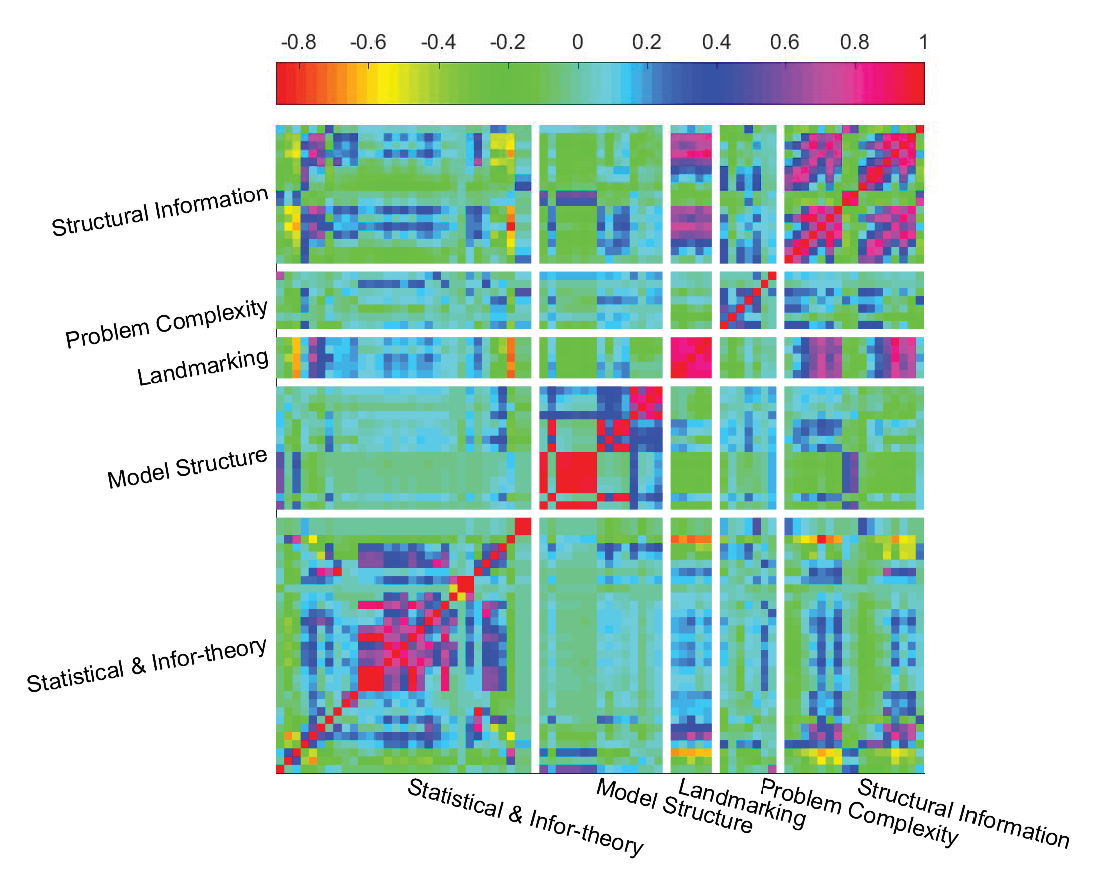
\includegraphics[width=0.75\textwidth]{Figures/CorrelationBetweenMetaFeatures}
    \caption{Correlation Coefficients among Five Different Kinds of Meta-features over 1723 Classification Problems}\label{Fig:CorrelationAmongMetaFeatures}
\end{figure}
%====================================================================
    \item Diverse base model construction

    There have been five different kinds of meta-features in the
    field of algorithm recommendation (See details in \cite{wang2014generic}). These meta-features are extracted
    from different viewpoints of a classification problem independently. So it is
    reasonable to assume that, different kinds of meta-features are independent
    with each other. Fig. \ref{Fig:CorrelationAmongMetaFeatures} gives the correlation
    coefficients among the five kinds of meta-features extracted from
    1723 benchmark classification problems. From this figure, we can
    find that the correlation among different kinds of meta-features is
    usually quite low. This gives us an experimental evidence that different kinds of
    meta-features are independent with each other.
    Furthermore, it is more likely that different recommendation models constructed with
    these different kinds of meta-features will be independent/diverse.
\end{enumerate}
%================================================================

\subsection{General View}\label{subsec:genView}

Firstly, different kinds of meta-features and the multi-labeled
meta-target are collected over a set of historical classification
problems; afterwards, by joining different combinations of these
meta-features and the multi-labeled meta-target together, different
sets of multi-labeled meta-data will be generated. Secondly, the
base recommendation models are constructed on each of the generated
multi-labeled meta-data. Thirdly, a multi-label ensemble learning
recommendation model will be achieved by combining these base
recommendation models together. Fig. \ref{Fig:ModelConstructProcess}
gives the general view of the proposed method which consists of
three steps: i) meta-data preparation, ii) base recommendation model
construction and iii) ensemble model construction.

%=================================================================
\begin{figure}
    \centering
    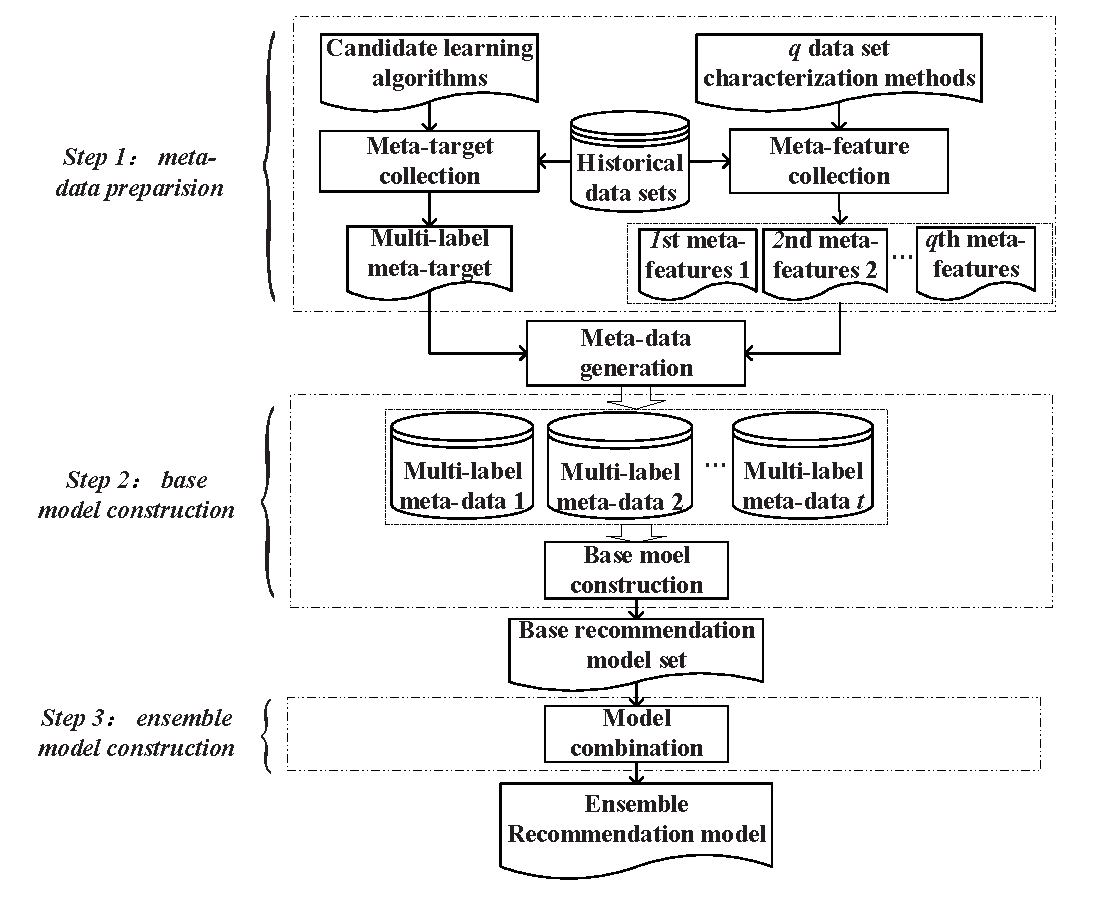
\includegraphics[width=0.75\textwidth]{Figures/MethodGeneralView3}
    \caption{General View of Ensemble based Classification Algorithm Recommendation Model Construction}\label{Fig:ModelConstructProcess}
\end{figure}
%=================================================================

\begin{enumerate}[1)]
    \item Meta-data preparation

    Meta-data is collected from a set of historical classification problems.
    i) For meta-feature collection, all the \emph{q} different kinds of data
    characterization methods are utilized on the historical classification problems to get \emph{q} groups of
    meta-features. ii) For meta-target collection, the
    appropriate algorithms of each historical classification problem are identified
    by statistically comparing all the candidate
    algorithms in terms of a given performance metric (e.g., classification accuracy).
    These appropriate algorithms form the multi-label based meta-target.

    \quad  Different kinds of meta-features reflect the properties of a
    classification problem in different viewpoints. Combinations of these
    meta-features will give us a more comprehensive understanding
    of the problem. Inspired by this idea, this paper attempts to
    construct the base recommendation models with respect to
    different combinations of these meta-features in a specific way. Firstly, \emph{q} different
    sets of meta-features can be combined to make out $\mathcal{T} = 2^q - 1$
    combinations (See the generation process in Section \ref{subsec:DataCollection}). Then, by merging these $\mathcal{T}$ combinations and
    the multi-labeled meta-target together, $\mathcal{T}$ different sets of multi-labeled meta-data can be
    generated.

    \item Base recommendation model construction

    For each multi-labeled meta data, firstly, the data transformation
    method is performed to transform the multi-labeled
    meta-data into multiple single-labeled meta-data, and then the
    base recommendation models will be generated on these
    single-labeled meta-data. The details of this process will be described in Section
    \ref{subsec:baseModel}.

    \item Ensemble recommendation model construction

    Once achieving the base recommendation models, the accurate and
    diverse base models are identified for constructing an ensemble
    recommendation model.
    For a new coming classification problem, the recommendations of
    these identified base models are combined in a specific way to form the
    recommended algorithms for the new problem. The detailed
    process of ensemble model construction will be introduced in
    Section \ref{subsec:ensembleModelConstruction}.
\end{enumerate}

\subsection{Meta-data Preparation}\label{subsec:DataCollection}

Let $\mathbb{A} = \{A_i: i = 1, 2, \cdots, k\}$ be a set of $k$
candidate classification algorithms, $\mathbb{P} = \{p_i: i = 1, 2,
\cdots, n\}$ be a set of $n$ historical classification problems, and
$F = \{F_i: i = 1, 2, \cdots, q\}$ be $q$ different data set
characterization functions used for meta-feature extraction.
$X_{i}^{j} = F_{j}(p_i)$ denotes the meta-features extracted by
$F_j$ ($1\leq j \leq q$) on the classification problem $p_i$ ($1\leq
i\leq n$).

Suppose that $D = \{(X_i, Y_i): i = 1, 2, \cdots, n\}$ denotes a set
of multi-label meta-instances, where $X_i$ is the meta-features
extracted from the classification problem $p_i$ by the function(s)
in $F$, that is, $X_i$ $\in$ $nchoosek(\{X_{i}^{1}$, $X_{i}^{2}$,
$\cdots$, $X_{i}^{q}\})$ and here $nchoosek(Z)$ outputs all the
possible combinations of the elements in $Z$. For example, let $Z =
\{a,b,c\}$, then $nchoosek(Z)$ = \{\{$a$\}, \{$b$\}, \{$c$\},
\{$a,b$\}, \{$a,c$\}, \{$b,c$\}, \{$a,b,c$\}\}; and $Y_i =
\{Y_{i,j}: j = 1, 2, \cdots, k\}$ represents the multi-label based
meta-target on $p_i$ and $Y_{i,j} =$ 1 or 0 indicates the algorithm
$A_j$ is appropriate or unappropriate on $p_i$.

It is noted that, there are many methods to generate different
combinations of meta-features from the given $q$ kinds of
meta-features. The combination function $nchoosek()$ being chosen is
due to the fact that it can not only generate multiple different
sets of meta-data for base model construction, but also help to find
whether the combinations of different kinds of meta-features are
better, and further discover the salient meta-features for algorithm
recommendation.

With the combination function $nchoosek()$ on $q$ different kinds of
meta-features, we can generate $\mathcal{T} = 2^q - 1$ different sets of
meta-features and furthermore $\mathcal{T}$ sets of multi-labeled meta-data.

\subsection{Base Recommendation Model Construction}\label{subsec:baseModel}

For each one of the $\mathcal{T}$ sets of multi-labeled meta-data, the process
to construct the base recommendation models is identical. This
section will illustrate this process by taking one given
multi-labeled meta-data $D^{(t)}$ ($1 \leq t \leq \mathcal{T}$) as an example.

At first, the multi-labeled meta-data $D^{(t)}$ is transformed into
multiple single-labeled data sets in meta-target space. The popular
data transformation method, Binary Relevance (BR)
\cite{tsoumakas2010mining}, is performed. The BR method transforms
$D^{(t)}$ into $k$ data sets $D_{j}^{(t)}, j= 1,\cdots,k$ which contain all
the instances of $D^{(t)}$ labeled by whether algorithm $A_j$ is
appropriate or not. This means, for each instance $(X_i^{(t)}, Y_i)$ of
$D^{(t)}$, the corresponding instance of $D_{j}^{(t)}$ is $(X_i^{(t)}, Y_{i,j})$.
Fig. \ref{Fig:dataTransformation} shows the $k$ binary
single-labeled data sets produced by BR on the multi-labeled
meta-data $D^{(t)}$.
%==================================================================
\begin{figure}[!h]
	\centering
	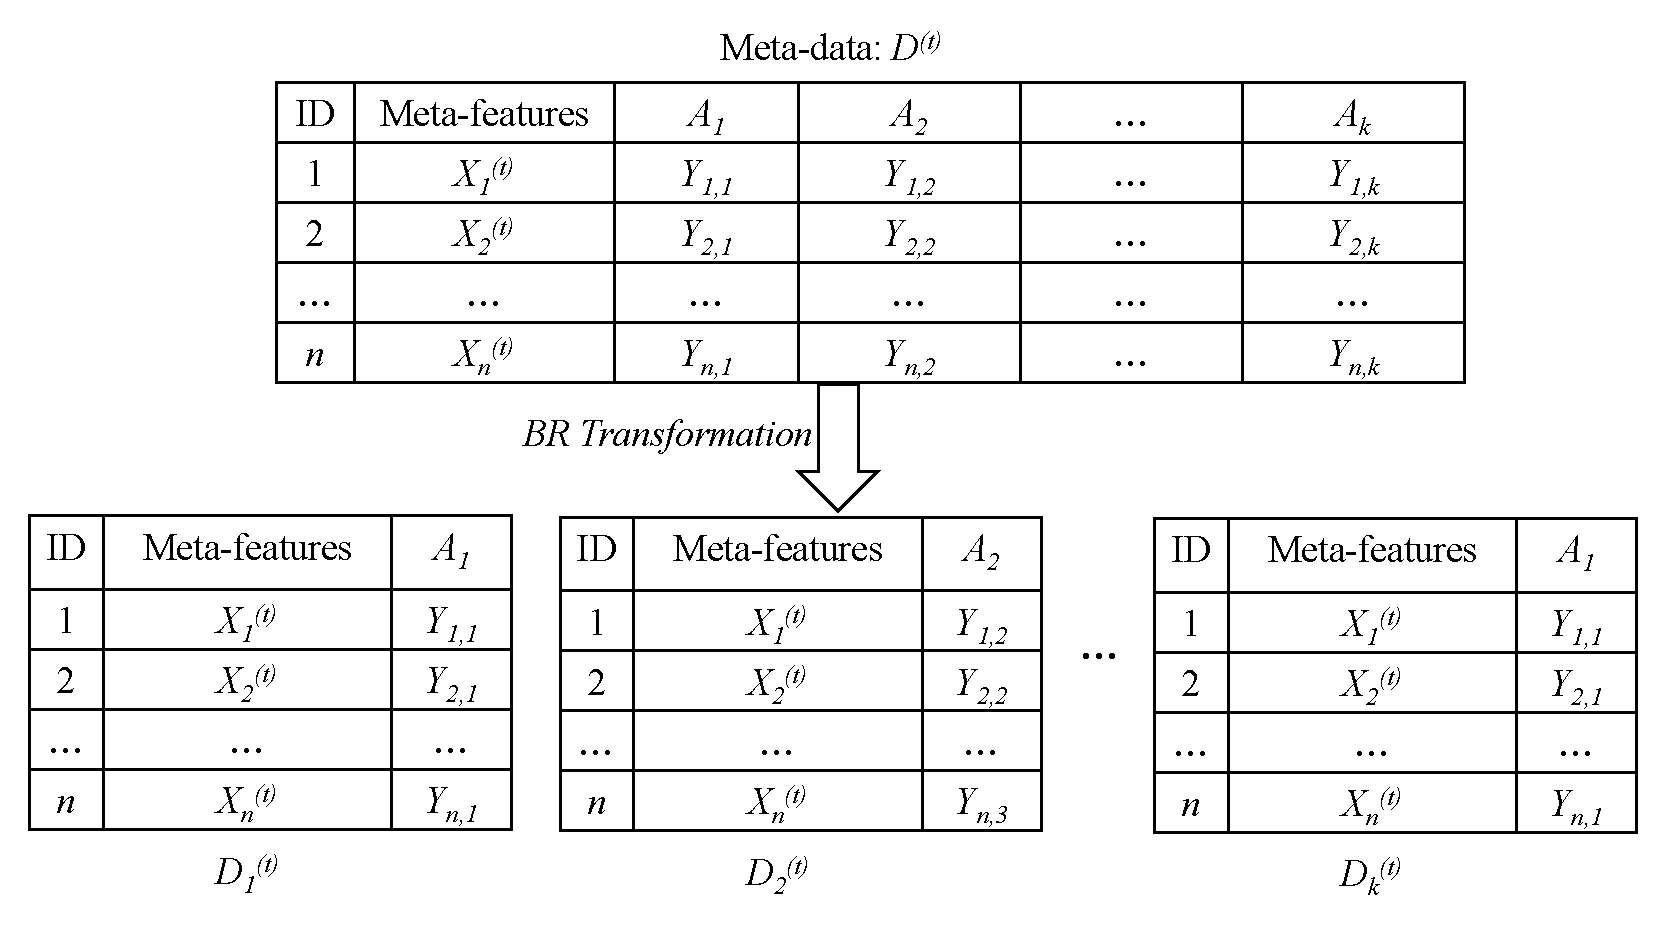
\includegraphics[width=0.7\textwidth]{Figures/DataTransformation}
	\caption{Schematic of Single-labeled Data Set Generation from Multi-label Meta Data $D^{(t)}$ by BR Method}\label{Fig:dataTransformation}
\end{figure}
%==================================================================

Afterwards, $k$ recommendation models will be learned on these $k$
binary learning data sets by a specific classification algorithm
(e.g, Decision Tree). These $k$ binary learning models constitute
the base recommendation models on $D^{(t)}$.

After constructing base recommendation models on each one of the $\mathcal{T}$
multi-labeled meta-data generated by combining the $q$ different
kinds of meta-features, we will get a recommendation model matrix
$M_{\mathcal{T}\times k}$, where $M_{i,j} (1\leq i\leq \mathcal{T}, 1\leq j \leq k)$
denotes the model learned on the $j$th data set transformed from
$i$th multi-labeled meta-data by BR method.

%==============================================================
\begin{equation}
    M_{\mathcal{T}\times k} =\left[
  \begin{array}{cccc}
    M_{1,1} & M_{1,2} & \cdots & M_{1,k} \\
    M_{2,1} & M_{2,2} & \cdots & M_{2,k} \\
    \vdots & \vdots &  \vdots & \vdots \\
    M_{\mathcal{T},1} & M_{\mathcal{T},2} & \cdots & M_{\mathcal{T},k} \\
  \end{array}
    \right]
\end{equation}
%==============================================================

Let $M_{\cdot,j} (1\leq j \leq k)$ denote the $j$th column of the
matrix $M_{\mathcal{T}\times k}$. According to the process of BR
transformation method, $M_{\cdot,j}$ consists of all the $\mathcal{T}$ binary
learning models with respect to the candidate algorithm $A_j$. Thus,
it is possible for us to construct the ensemble learning model
improve the recommendation of $A_j$ based on these $\mathcal{T}$ models in
$M_{\cdot,j}$.

\subsection{Ensemble Recommendation Model Construction}\label{subsec:ensembleModelConstruction}

As the accurate and diverse base models play a critical role in
constructing an ensemble recommendation model, in this section, we
first give the definitions of accurate and diverse base
recommendation models from the view of ensemble learning.
Afterwards, based on these definitions, we identify a set of
accurate and diverse base recommendation models for ensemble.

\subsubsection{Definitions of Accurate and Diverse Learning Models}\label{subsubsec:accurateAndDiverseModel}

Let $M_{E}$ be an ensemble learning model constructed with $n$
binary learning models \{$M_1$, $M_2$, $\cdots$,
$M_n$\}\footnote{All the base models are binary classification
models since we transform the multi-labeled meta-data into multiple
single-labeled binary meta-data.}, and $pr_{M_i}$ ($1\leq i\leq n$)
be the probability of $M_{i}$ to make an error prediction on a new
coming instance. Then, for ensemble learning, according to the research in \cite{dietterich2000ensemble}, an accurate learning model can be defined as follow.

\begin{definition}\textbf{Accurate learning model}\label{def:accurateModel}.
A base learning model $M_i$ ($1\leq i\leq n$) is accurate if and
only if $pr_{M_i} < 1/2$.
\end{definition}

Definition \ref{def:accurateModel} tells us that a base learning
model is accurate if and only if its prediction error is less than
1/2.

Without the independence/diversity among the base models \{$M_1,
M_2, \cdots, M_n$\}, the prediction error of the ensemble model $M_{E}$
will be no-converging or converging too slowly to a low value. This
phenomenon has been recognized in learner combination
\cite{cunningham2000diversity,lam2000classifier}. The diverse
ensemble learner has a better potential to improve the accuracy than
non-diverse ensemble leaner
\cite{peterson2005estimating,brown2005diversity,kuncheva2003measures}.
Therefore, there will be a notable question: ``How to define or
evaluate the independence/diversity among the base learning
models?''.

In the field of ensemble learning, it is usually difficult to
evaluate the diversity between different learning models directly.
Researchers usually resort to the prediction/classifcation results
of the learning models on a given test data. There have been several
metrics proposed based on the prediction results to assess the
diversity between different models
\cite{kuncheva2003measures,lee2013automatic,cunningham2000diversity,dietterich2000experimental}.
These metrics can guide us to identify the diverse base models.
Meanwhile, \cite{kuncheva2003measures} have stated that, in order to
guaranteed the improvement over the performance of base models,
there exists a minimum threshold value for each of these diversity
metrics to pick up the diverse base models for ensemble learning.

Following these ideas, suppose that $M_i$ and $M_j$ ($1\leq i\neq\j
\leq n$) are two different base models, and $R_i$ and $R_j$ are the
predicstion/classification results of $M_i$ and $M_j$ on a given
test data set $D$, we can give the definition of diverse learning
model for ensemble learning as follow.

\begin{definition}\textbf{Diverse learning model}\label{def:diverseModel}.
Two base models $M_i$ and $M_j$ are diverse with each other if and
only if $\psi(R_i, R_j) < \delta$, where $\psi$ is a function which
computes the diversity between $M_i$ and $M_j$ based on $R_i$ and
$R_j$, and $\delta$ is a given minimum threshold.
\end{definition}

In the field of ensemble learning, the
researchers usually define the diversity function $\psi$ in terms of
either class label or correct/incorrect decision
\cite{kohavi1996bias,dietterich2000experimental,Ho1998Random,Giacinto2000design,kuncheva2003measures}.
In this paper, we propose a function, which makes full use of the
prediction results and considers both of the class label and
correct/incorrect decision, to pick up the diverse models for
ensemble.

Suppose there are two different learning models $M_1$ and $M_2$, and
a data set $D$ with $K$ class labels \{$C_1$, $C_2$, $\cdots$,
$C_K$\} (for algorithm recommendation in this paper, $K =
2$)\footnote{The method to identify the diverse learning models is
not limited to binary classification but also appropriate for
multi-classification, i.e., $K > 2$.}, then we can construct a $K\times K$ contingency table (see
Table \ref{table:contingencyTable}) based on the class labels and
correct/incorrect decisions predicted by $M_1$ and $M_2$ on $D$.

%================================================================
\begin{table}[!h]
    \caption{The $K\times K$ Contingency Table of Two Learning Models}\label{table:contingencyTable}
    \centering
    \resizebox{0.45\textwidth}{!}{
    \begin{tabular}{c | c c c c |c}
    \hline
    Classified label & $C_1$ & $C_2$ & $\cdots$ & $C_K$ & Total \\
    \hline
    $C_1$ & $N_{1,1}$ & $N_{1,2}$ & $\cdots$ & $N_{1,K}$ & $N_{1,*}$\\
    $C_2$ & $N_{2,1}$ & $N_{2,2}$ & $\cdots$ & $N_{2,K}$ & $N_{2,*}$\\
    $\vdots$ & $\vdots$ & $\vdots$ & $\vdots$ & $\vdots$ & $\vdots$\\
    $C_K$ & $N_{K,1}$ & $N_{K,2}$ & $\cdots$ & $N_{K,K}$ & $N_{K,*}$\\
    \hline
    Total & $N_{*,1}$ & $N_{*,2}$ & $\cdots$ & $N_{*,K}$ & $N$\\
    \hline
    \end{tabular}
    }
\end{table}
%===========================================================================

In Table \ref{table:contingencyTable}, $N_{i,j}$ ($1\leq i, j\leq
K$) is the number of test instances incorrectly classified as $C_i$
and $C_j$ by $M_1$ and $M_2$, respectively. $N_{i,*} =
\sum_{j = 1}^{K}N_{i,j}$ ($1\leq i\leq K$), $N_{*,j} =
\sum_{i = 1}^{K}N_{i,j}$ ($1\leq j\leq K$) and $N =
\sum_{i=1}^{K}N_{i,*} = \sum_{j=1}^{K}N_{*,j} =
\sum_{i=1}^{K}\sum_{j=1}^{K}N_{i,j}$. $N$ is the total
number of instances of $D$ which are incorrectly predicted by either
$M_1$ or $M_2$.

With this $K\times K$ contingency table, we can get the diverse
measure $\kappa$ by Eq. \ref{eq:kappa}. The greater the value of
$|\kappa|$, the smaller the diversity between $M_1$ and $M_2$.

%==============================================================
\begin{equation}\label{eq:kappa}
    \kappa = \frac{\Theta_1 - \Theta_2}{1 - \Theta_{2}}.
\end{equation}
%==============================================================

Where $\Theta_1 = \sum\limits_{i=1}^{K}\frac{N_{i,i}}{N}$ and
$\Theta_2 =
\sum\limits_{i=1}^{K}\frac{N_{i,*}}{N}\times\frac{N_{*,i}}{N}$.

According to the contingency table analysis, the joint frequency
distribution of $C_i$ and $C_j$ predicted by $M_1$ and $M_2$ is
$\frac{N_{i,j}}{N}$, and $\frac{N_{i,*}}{N}$ and $\frac{N_{*,j}}{N}$
correspond to the marginal frequency distributions of $C_i$ and
$C_j$.

In practical application, the metric $\kappa$ is estimated via the
prediction results of the learning models on only a sample rather
than the whole population. This might also be the reason that there
needs a threshold $\delta$ in Definition \ref{def:diverseModel}.
Therefore, we need to further understand the statistical
significance of $\kappa$, including the statistical significance of
$\kappa\neq 0$ and its confidence interval. And the confidence
interval will be set as the threshold $\delta$ in Definition
\ref{def:diverseModel}.

For this purpose, we need to find a statistic for significant test
of $\kappa$. As we know, the distribution of the class labels
predicted by a learner on a $K-class$ classification problem would
follow either binomial ($K = 2$) or multi-nominal ($K > 2$)
distribution. Both of binomial, multi-nominal distributions are
derived from exponential family of distributions. Meanwhile,
inspired by the idea that the independence between two variables,
which follow the well-known exponential distribution (i.e, normal
distribution), is usually statistically tested by a $t$-statistic,
we attempt to employ a $t$-statistic in Eq. \ref{eq:tstatisc} to
test the significance of $\kappa \neq 0$, and further determine
whether two learning models $M_1$ and $M_2$ are independent with
each other or not.

%=================================================================
\begin{equation}\label{eq:tstatisc}
    t = \frac{\kappa}{\sqrt{\frac{1-\kappa^2}{N-2}}}
\end{equation}
%=================================================================

The $t$ statistic follows the Student's t-distribution with freedom
of degree $N-2$ under the null hypothesis that $M_1$ and $M_2$ are
independent with each other. If the $t$-statistic test accepts the
null hypothesis under given significance level $\alpha$, we can
conclude that the measure $\kappa$ has no significant difference
with 0, i.e., $M_1$ and $M_2$ are independent with each other.

According to Eq. \ref{eq:tstatisc}, its inverse can be calculated as
follow
\begin{equation}\label{eq:tinver}
    \kappa = \frac{t}{\sqrt{N - 2 + t^2}}
\end{equation}
Where $t$ statistic follows student distribution with degree of
freedom $N-2$.

Let $t_{c}$ denote the critical value of student distribution with
degree of freedom $N-2$ under a given significance level $\alpha$
(e.g., $\alpha$ = 0.05), then we can get the confidence interval of
$\kappa = 0$ as $[-\frac{t_c}{\sqrt{N - 2 + t_c^2}},
\frac{t_c}{\sqrt{N - 2 + t_c^2}}]$. If $\kappa$ calculated between
two single learning models falls into this interval, we can conclude
that these two models are statistically independent with each other
under the given significance level $\alpha$. Based on this
confidence interval, we can set the minimum threshold $\delta =
\frac{t_c}{\sqrt{N - 2 + t_c^2}}$. And the diverse models can be
detected by comparing $\kappa$ with $\delta$ directly. That is, two
models $M_1$ and $M_2$ are independent with each other if and only
if $|\kappa| < \delta$.


\subsubsection{Combination of Base Recommendation
Models}\label{subsubsec:ensembleRecommendation}

According to Corollary \ref{coro:condition}, the necessary and
sufficient condition of constructing an accurate ensemble
recommendation model is that the base models are accurate and
diverse with each other. Thus, the ensemble recommendation model
construction is a process to find out the accurate and diverse
models in $M_{\cdot,j} = \{M_{1,j}, M_{2,j}, \cdots, M_{\mathcal{T},j}\}$.

%================================================================
\IncMargin{0.35em} \RestyleAlgo{ruled}\LinesNumbered
\begin{algorithm}[!ht]
  \scriptsize
  \SetAlgoVlined
  \caption{ModelFilter()}\label{algo:modelFilter}
  %=========================================================
  \SetKwInOut{Input}{Inputs}
  \SetKwInOut{Output}{Output}
  \SetKwComment{tcc}{/*}{*/}
  \SetKwComment{rcc}{//}{}
  %=========================================================
 \Input{
    $M_{\cdot,j} = \{M_{1,j}, M_{2,j}, \cdots, M_{\mathcal{T},j}\}$\;
    \hspace{1.3cm} $Accs = \{acc_1, acc_2, \cdots, acc_\mathcal{T}\}$\;
    \hspace{1.3cm} $Outs = \{out_1, out_2, \cdots, out_\mathcal{T}\}$;
 }
%=========================================================
 \BlankLine
 \Output{ $FlagList = \{f_1, f_2, \cdots, f_\mathcal{T}\}$;}
%=========================================================
 \BlankLine
 Initialization: $\{f_i = 1: (1\leq i\leq \mathcal{T})\}$\;
 \rcc{Part 1: Accuracy based filter}
 \For{$i = 1$ \KwTo $\mathcal{T}$} {
    \If{$acc_i < 0.5$}{
        $f_i = 0$;
    }
 }
 \rcc{Part 2: Diversity based filter}
 $IX$ = sort($Accs$, ``descend'')\rcc{$IX$ is the indices of the models sorted by $Accs$ in a descending order}
 \For{$i = 1$ \KwTo $\mathcal{T}-1$} {
    $Idi$ = $IX_i$;\rcc{The $i$th element of $IX$}
    \If{$f_{Idi} == 1$}{
        \For{$j = (i+1)$ \KwTo $\mathcal{T}$} {
            $Idj$ = $IX_j$\rcc{The $j$th element of $IX$}
            \If{$f_{Idj} == 1$}{
                $\kappa$ = DiversityComp($Out_{Idi}$, $Out_{Idj}$)\rcc{According to Eq. \ref{eq:kappa} of $\kappa$}
                \If{$\kappa \geq \delta$}{
                    $f_{Idj} = 0$;\rcc{$\delta$ is set according to Eq. \ref{eq:tinver}}
                }
            }
        }
    }
 }
\end{algorithm}
\DecMargin{0.35em} \LinesNumbered
%================================================================

Algorithm \ref{algo:modelFilter} gives a filtering method on the $\mathcal{T}$
base recommendation models in $M_{\cdot,j}$. In this algorithm,
besides $M_{\cdot,j}$, there are two other input variables $Accs$
and $Outs$ with respect to the learning models in $M_{\cdot,j}$. Due
to the fact that each model $M_{i,j}$ is constructed on a binary
single-label learning data set generated by BR transformation, we
can get that $acc_i \in Accs$ ($1\leq i \leq \mathcal{T}$) denotes the
classification accuracy of $M_{i,j}$ on a validation data
set\footnote{The validation data set is drawn from the original
meta-data and never used for model construction.}, and $out_i \in
Outs$ represents the outputs (i.e., predicted labels and
correct/incorrect decisions) of $M_{i,j}$ on the validation data.
The concepts of classification accuracy, predicted labels and
correct/incorrect decisions are consistent with those in traditional
single-label learning. The output $FlagList$ records the filtering
results, where $f_i \in \{0,1\}$ and $f_i = 0/1$ means that
$M_{i,j}$ is filtered out/reserved for ensemble model construction.

Algorithm \ref{algo:modelFilter} consists of two filters: i)
accuracy based filter (lines 2-3) and ii) diversity based filter
(lines 5-14). The first filter is used to find out the accurate base
recommendation models. In this filter, the models whose
classification accuracy being smaller than 1/2 are filtered out
(i.e., set the corresponding flags in $FlagList$ as 0) according to
Definition \ref{def:accurateModel} of accurate model. The second
filter aims at finding out the diverse models. In this filter, if
the $\kappa$ between two specified models is greater than the
predefined threshold $\delta$ according to Definition
\ref{def:diverseModel} of diverse model, the model with lower
classification accuracy will be filtered out. Where the threshold
$\delta$ is set according to Eq. \ref{eq:tinver}.

With the help of Algorithm \ref{algo:modelFilter}, we can get a flag
matrix $G_{\mathcal{T}\times k}$, where the column $f_{\cdot,j} (1\leq j\leq
k)$ is achieved by applying Algorithm \ref{algo:modelFilter} on the
models $M_{\cdot, j}$ of the $j$th column in the model matrix
$M_{\mathcal{T}\times k}$, $f_{i,j} \in \{0,1\}$ ($1\leq i\leq \mathcal{T}$), and
$f_{i,j} = 1$ means the model $M_{i,j}$ is chosen for ensemble model
construction.

%==============================================================
\begin{equation}
    G_{\mathcal{T}\times k} =\left[
  \begin{array}{cccc}
    f_{1,1} & f_{1,2} & \cdots & f_{1,k} \\
    f_{2,1} & f_{2,2} & \cdots & f_{2,k} \\
    \vdots & \vdots &  \vdots & \vdots \\
    f_{\mathcal{T},1} & f_{\mathcal{T},2} & \cdots & f_{\mathcal{T},k} \\
  \end{array}
    \right]
\end{equation}
%==============================================================

Meanwhile, let $M_{i,\cdot} (1\leq i\leq \mathcal{T})$ be the $i$th row of the
model matrix $M_{t,k}$, which consists of the models learned from
the $i$th multi-labeled meta-data. For a new coming classification
problem $p_{new}$, each model $M_{i,j} \in M_{i,\cdot}$ ($1\leq
j\leq k$) predicts the probability $pr_{i,j}$ to recommend the
algorithm $A_j$ to $p_{new}$. So we can further get a matrix
$P_{\mathcal{T}\times k}$ of probabilities predicted by the model matrix
$M_{\mathcal{T}\times k}$ on $p_{new}$ as follow.

%==============================================================
\begin{equation}
    P_{\mathcal{T}\times k} =\left[
  \begin{array}{cccc}
    pr_{1,1} & pr_{1,2} & \cdots & pr_{1,k} \\
    pr_{2,1} & pr_{2,2} & \cdots & pr_{2,k} \\
    \vdots & \vdots &  \vdots & \vdots \\
    pr_{\mathcal{T},1} & pr_{\mathcal{T},2} & \cdots & pr_{\mathcal{T},k} \\
  \end{array}
    \right]
\end{equation}
%==============================================================

With the predicted probability value matrix $P_{\mathcal{T}\times k}$ and the
flag matrix $G_{\mathcal{T}\times k}$, the ensemble recommendation model will
estimate the probability value of the candidate algorithm $A_j
(1\leq j\leq k)$ being appropriate on $p_{new}$ by the Eq.
\ref{eq:ensemPro}.

%===============================================================
\begin{equation}\label{eq:ensemPro}
    pr_{en}(A_j) = \frac{\sum\limits_{i=1}^{\mathcal{T}}pr_{i,j}\cdot f_{i,j}}{\sum\limits_{i=1}^{\mathcal{T}}f_{i,j}}
\end{equation}
%===============================================================

In Eq. \ref{eq:ensemPro}, the denominator
$\sum\limits_{i=1}^{\mathcal{T}}f_{i,j}$ denotes the number of models chosen
by Algorithm \ref{algo:modelFilter} on $M_{\cdot,j}$, i.e., the
number of based models used for ensemble learning with respect to
algorithm $A_j$. The molecule of Eq. \ref{eq:ensemPro} can be viewed
as a kind of weighted voting ensemble, where $pr_{i,j}$ denotes the
weight of model $M_{i,j}$ and it works if and only if $f_{i,j} = 1$,
i.e., $M_{i,j}$ is picked up as a base model for ensemble learning.

Afterwards, the ensemble recommendation model can rank the $k$
candidate algorithms according to the estimated probability values
$\{pr_{en}(A_1)$, $pr_{en}(A_2)$, $\cdots$, $pr_{en}(A_k)\}$.
Meanwhile, the algorithm $A_j$ will be recommended as an appropriate
one for $p_{new}$ if and only if $pr_{en}(A_j)$ is greater than a
specific threshold (e.g., 1/2).

%================================================================
\begin{table}[!h]
    \caption{Example for Ranking Strategy}\label{table:RankExample}
    \centering
    \scriptsize
    \resizebox{0.75\textwidth}{!}{
    \begin{tabular}{l c c c c c}
    \hline
    Algorithm & $A_1$ & $A_2$ & $A_3$ & $A_4$ & $A_5$ \\
    \hline
    Probability value & 0.7 & 0.4 & 0.8 & 0.5 & 0.7 \\
    Ranks & 2 & 5 & 1 & 4 & 3 \\
    Ranks (considering ties) &2.5 & 5 & 1 & 4 & 2.5\\
    \hline
    \end{tabular}
    }
\end{table}
%===========================================================================

Meanwhile, these $k$ probability values can be further used to learn
a ranking list of the candidate algorithms in $\mathbb{A}$ on
$p_{new}$. The algorithm with the highest probability will be ranked
first, the algorithm with the second highest probability will be
ranked second, and so on. In case of ties, average ranks are
assigned. This strategy can be illustrated by the example in Table
\ref{table:RankExample} in which we give the estimated probability
values of five candidate algorithms and corresponding ranks.

\section{Experimental Study}\label{sec:ExpStudy}
In this section, we experimentally evaluate the performance of the
proposed ensemble learning based algorithm recommendation method,
including the experimental setup and analyses of the results\footnote{The meta-data of all the classification problems and the source codes of ensemble multi-label learning based algorithm recommendation are available on website \url{http://cn.mathworks.com/matlabcentral/fileexchange/57716-classification-algorithm-automatic-recommendation}}.

%===========================================================================
\begin{table}[!h]
    \caption{Description of the 112 Classification Problems}\label{table:dataset}
    \centering
    \resizebox{0.65\textwidth}{!}{
    \begin{threeparttable}
    \begin{tabular}{l l l l l | l l l l l}
    \hline
    ID  &  Name & F & I & C & ID  &  Name & F & I  & C \\
    \hline
1 & anneal & 38 & 898 & 6 & 57 & page-blocks & 10 & 5473 & 5\\
2 & anneal.ORIG & 38 & 898 & 6 & 58 & pendigits & 16 & 10992 & 10\\
3 & arrhythmia & 279 & 452 & 16 & 59 & pima & 6 & 768 & 2\\
4 & audiology & 69 & 226 & 24 & 60 & post-pat-data & 8 & 90 & 3\\
5 & australian & 14 & 690 & 2 & 61 & primary-tumor & 17 & 339 & 22\\
6 & autos & 25 & 205 & 7 & 62 & segment & 19 & 2310 & 7\\
7 & balance-scale & 4 & 625 & 3 & 63 & shut-land-con & 6 & 15 & 2\\
8 & breast-cancer & 9 & 286 & 2 & 64 & sick & 29 & 3772 & 2\\
9 & breast-w & 9 & 699 & 2 & 65 & solar-flare\_1 & 12 & 323 & 2\\
10 & car & 6 & 1728 & 4 & 66 & solar-flare\_2 & 12 & 1066 & 3\\
11 & cleve & 11 & 303 & 2 & 67 & sonar & 60 & 208 & 2\\
12 & cmc & 9 & 1473 & 3 & 68 & soybean & 35 & 683 & 19\\
13 & colic & 22 & 368 & 2 & 69 & spambase & 57 & 4601 & 2\\
14 & connect-4 & 42 & 13512 & 3 & 70 & spect & 22 & 267 & 2\\
15 & credit-a & 15 & 690 & 2 & 71 & spectrometer & 102 & 531 & 48\\
16 & credit-g & 20 & 1000 & 2 & 72 & splice & 61 & 3190 & 3\\
17 & crx & 15 & 690 & 2 & 73 & sponge & 45 & 76 & 3\\
18 & cylinder-bands & 39 & 540 & 2 & 74 & tae & 5 & 151 & 3\\
19 & dermatology & 34 & 366 & 6 & 75 & tic-tac-toe & 9 & 958 & 2\\
20 & diabetes & 8 & 768 & 2 & 76 & trains & 32 & 10 & 2\\
21 & ecoli & 7 & 336 & 8 & 77 & transfusion & 3 & 748 & 2\\
22 & flags & 29 & 194 & 8 & 78 & vehicle & 18 & 846 & 4\\
23 & german & 15 & 1000 & 2 & 79 & vote & 16 & 435 & 2\\
24 & glass & 9 & 214 & 7 & 80 & vowel & 13 & 990 & 11\\
25 & haberman & 3 & 306 & 2 & 81 & waveform-5000 & 40 & 5000 & 3\\
26 & hayes-roth & 4 & 132 & 3 & 82 & wine & 13 & 178 & 3\\
27 & heart-c & 13 & 303 & 5 & 83 & yeast & 7 & 1484 & 10\\
28 & heart-h & 13 & 294 & 5 & 84 & zoo & 17 & 101 & 7\\
29 & heart-statlog & 13 & 270 & 2 & 85 & ALLAML & 7130 & 72 & 2\\
30 & hepatitis & 19 & 155 & 2 & 86 & arcene & 10001 & 200 & 2\\
31 & horse-colic.ORIG & 21 & 368 & 2 & 87 & BASEHOCK & 4863 & 1993 & 2\\
32 & hypo & 23 & 3163 & 2 & 88 & Carcinom & 9183 & 174 & 11\\
33 & hypothyroid & 29 & 3772 & 4 & 89 & CLL\_SUB\_111 & 11341 & 111 & 3\\
34 & ionosphere & 34 & 351 & 2 & 90 & COIL20 & 1025 & 1440 & 20\\
35 & iris & 4 & 150 & 3 & 91 & colon & 2001 & 62 & 2\\
36 & kdd\_JapVow\_1 & 14 & 5687 & 9 & 92 & gisette & 5001 & 7000 & 2\\
37 & kdd\_JapVow\_2 & 13 & 4274 & 9 & 93 & GLIOMA & 4435 & 50 & 4\\
38 & kdd\_syn\_con & 61 & 600 & 6 & 94 & GLI\_85 & 22284 & 85 & 2\\
39 & kr-vs-kp & 36 & 3196 & 2 & 95 & Isolet & 618 & 1560 & 26\\
40 & labor & 16 & 57 & 2 & 96 & leukemia & 7071 & 72 & 2\\
41 & led7 & 7 & 3200 & 10 & 97 & lung & 3313 & 203 & 5\\
42 & letter & 16 & 20000 & 26 & 98 & lymphoma & 4027 & 96 & 9\\
43 & liver-disorders & 6 & 345 & 2 & 99 & madelon & 501 & 2600 & 2\\
44 & lung-cancer & 56 & 32 & 3 & 100 & nci9 & 9713 & 60 & 9\\
45 & lymph & 18 & 148 & 4 & 101 & ORL & 1025 & 400 & 40\\
46 & mfeat-fourier & 76 & 2000 & 10 & 102 & orlraws10P & 10305 & 100 & 10\\
47 & mfeat-karhunen & 64 & 2000 & 10 & 103 & PCMAC & 3290 & 1943 & 2\\
48 & mfeat-morphological & 6 & 2000 & 10 & 104 & pixraw10P & 10001 & 100 & 10\\
49 & mfeat-zernike & 47 & 2000 & 10 & 105 & Prostate\_GE & 5967 & 102 & 2\\
50 & mole-bio\_pro & 58 & 106 & 2 & 106 & RELATHE & 4323 & 1427 & 2\\
51 & monks-pro-1 & 6 & 556 & 2 & 107 & SMK\_CAN\_187 & 19994 & 187 & 2\\
52 & monks-pro-2 & 6 & 601 & 2 & 108 & TOX\_171  & 5749 & 171 & 4\\
53 & monks-pro-3 & 6 & 554 & 2 & 109 & USPS & 257 & 9298 & 10\\
54 & mushroom & 22 & 8124 & 2 & 110 & warpAR10P  & 2401 & 130 & 10\\
55 & nursery & 8 & 12960 & 5 & 111 & warpPIE10P & 2421 & 210 & 10\\
56 & optdigits & 64 & 5620 & 10 & 112 & Yale & 1025 & 165 & 15\\
    \hline
    \end{tabular}
        \begin{tablenotes}
            \footnotesize
            \item [$\ast$] ``F'' = number of features;
            ``I'' = number of instances; ``C'' = number of class values.
        \end{tablenotes}
    \end{threeparttable}
    }
\end{table}
%===========================================================================
\subsection{Experimental Setup}

In order to evaluate the effectiveness of the ensemble learning
based algorithm recommendation method, confirm the applicability in
practice, and guarantee the reproducibility of the results, we set
up our experiments as follows.

\subsubsection{Benchmark Classification Problem}

112 extensively-used public classification problems being available
on UCI
repository\footnote{\url{http://archive.ics.uci.edu/ml/datasets.html.}} and scikit-feature selection repository\footnote{\url{http://featureselection.asu.edu/index.php.} These data sets cover different domains, such as text, image, handwrite, biology and so on.}
are employed in the experiments. Table \ref{table:dataset} shows the
statistical summary of these problems in terms of the number of
attributes, the number of instances and the number of classes. The first 84
classification problems have also been used for constructing the
algorithm recommendation model in \cite{wang2014generic}.

Moreover, in order to guarantee the reliability and soundness of the
conclusion, more classification problems should be employed. Thus,
with the help of the problem generation method, Datasetoids, which
was proposed in \cite{soares2009uci} and aimed to obtain a large
number of classification problems for algorithm recommendation
\cite{prudencio2011selecting}, we extend the 112 publicly UCI
classification problems into 1723 (112 data sets and 1611
datasetoids) different classification problems. The Datasetoids
method is quite simple, it achieves the new classification problems
by exchanging role of each nominal attribute with that of a target
concept, i.e., viewing the nominal attribute as the new target
concept.

\subsubsection{Meta-feature Collection}

Five different types of meta-features are extracted from the 1723
classification problems. They are i) the statistical and
information-theory based, ii) the model structure based, iii) the
landmarking based, iv) the problem complexity based and v) the
structural information based. See Appendix \ref{appendix:metaFeature} for the details.

\subsubsection{Meta-target Collection}

Meta-target tells us that the appropriate candidate algorithms for
each of the 1723 classification problems. Next, we introduce the
candidate classification algorithms in the experiments and how to
identify the appropriate algorithms for a given classification
problem.

\begin{enumerate}
    \item \emph{Candidate classification algorithms}

    In order to guarantee the generality of the experimental
    results, 17 different types of classification algorithms are picked up
    as the candidates.

    \quad These algorithms include i) the probability based algorithms Naive Bayes and Bayes Network;
    ii) tree based algorithms C4.5, RandomTree, Gradient Boosting Decision tree (GBDT) and RandomForest; iii) lazy learning based $k$-Nearest Neighbors; iv)
    rule-based algorithms PART, Ripper and NNge; v) function based Logistic regression and RBFNetwork, and vi) support vector machine based algorithm SMO.

    \quad Besides the above classification algorithms, we also pick up two kinds of well-known
    ensemble classification algorithms: Boosting and Bagging. They are applied with the base
    classifiers Naive Bayes (NB) and C4.5, respectively.

    \item \emph{Appropriate algorithm identification}

    The multi-label based meta-target indicating the appropriate algorithms for a classification
    problem $P$ can be expressed in terms of a binary value vector $B_{P} = <b_1, b_2,
    \cdots, b_{17}>$, where $b_i = 1$ means that the corresponding candidate
    algorithm $A_i$ ($1\leq i\leq 17$) is appropriate. The appropriate algorithms are
    identified by their performance metrics (i.e., classification accuracy) on $P$ as follows.

    \begin{enumerate}
        \item {Process of classification accuracy estimation on $P$}

        In order to get a stable estimation of classification accuracy of
        the candidate algorithms on $P$, $5\times10$-fold stratified cross-validation is performed as
        the following steps. i) The problem $P$ is randomly split into ten mutually
        exclusive subsets $P_1, P_2, \cdots, P_{10}$ of equal size, and
        $P = \bigcup_{j=1}^{10} P_j$. ii) $P - P_j$ and $P_j$ ($j \in
        \{1,2,\cdots,10\}$) are used as the training and test sets, respectively.
        Each algorithm $A_i$ ($1\leq i \leq 17$)
        is trained on $P - P_j$, and its classification
        accuracy is estimated on $P_j$. iii) Repeat i) and ii) five times
        on $P$ whose instances are randomly re-ordered. Afterwards,
        for each candidate algorithm $A_i$ ($1\leq i \leq 17$),
        we will get a vector $Acc_i$ = $<acc_{i,1}$, $acc_{i,2}$,
        $\cdots$, $acc_{i,50}>$ with 50 classification accuracies.

        \item{Binary-valued based meta-target $B_{P}$ identification}

        In order to identify the real appropriate algorithms from
        17 candidate algorithms according to from the
        collected performance sets $\{Acc_1$, $Acc_2$, $\cdots$, $Acc_{17}\}$ on $P$,
        the statistical algorithm selection is a reasonable and commonly-used approach
        \cite{pizarro2002multiple}.

        \quad To find out the superior algorithms from three or
        more candidate algorithms, the traditional statistical methods
        usually resort to multiple paired \emph{t}-tests. However, it has
        been proved that this approach usually leads to high Type I
        error.\footnote{The probability that we make a mistake to reject the
        null hypothesis, i.e., a misjudgement to say there exists
        significant difference but actually does not.}

        \quad For solving this problem, we turn to the \emph{multiple comparison
        procedure}. The multiple comparison procedure is a statistical test
        technique which helps us compare three or more groups of metrics
        (e.g., classification accuracy) while controlling the probability to make the statistical Type I
        error \cite{pizarro2002multiple}. Moreover, it allows us to concern with a
        set of candidate algorithms not significantly different from the best one
        rather than a single algorithm. Therefore, the multiple comparison procedure is
        an effective method for multi-labeled meta-target collection.

        \quad Therefore, in our experiment, as suggested in \cite{demvar2006statistical}, we employ
        the non-parametric multiple comparison procedure, Friedman followed by Holm's
        procedure test, to obtain the binary-value based meta-target $B_{P}$ for the problem
        $P$ according to $\{Acc_1, Acc_2, \cdots, Acc_{17}\}$ as follows.
        \begin{enumerate}
            \item Applying Friedman test on $\{Acc_1$, $Acc_2$, $\cdots$, $Acc_{17}\}$, the
            null hypothesis of Friedman test is there does not exist
            significant difference among these 17 algorithms. If the result
             of the test support the null hypothesis, all these 17 algorithms
            will be viewed as the appropriate ones. This means that $\forall
            b_i$ of $B_{P}$ ($1\leq i\leq 17$), $b_i = 1$. And the multiple
            comparison procedure is over.

            \item Otherwise, there will exist significant
            difference among these candidate algorithms. In this case, we should apply
            the post-hoc Holm's procedure test to further find the real
            appropriate algorithms. At first, the algorithm with the
            highest average classification accuracy is picked up as a reference.
            The Holm's procedure test is performed to identify the appropriate
            algorithms from the rest ones. The algorithms that have no significant
            difference with the reference are viewed as the appropriate
            ones. Of course, the reference is an appropriate one as
            well. Afterwards, for each value $b_i (1\leq i\leq 17)$ in $B_{P}$, if the corresponding
            algorithm $A_i$ is identified as an appropriate one, $b_i = 1$,
            otherwise, $b_i = 0$.
        \end{enumerate}
    \end{enumerate}
\end{enumerate}

\subsubsection{Recommendation Model Construction}

The proposed ensemble multi-label learning based recommendation
model combines a set of base models constructed on different sets of
meta-data. In order to demonstrate whether the proposed ensemble
method is competitive in constructing the recommendation model, we
compare the performance of the ensemble recommendation model with
those of the base models.

When constructing the base model on a given multi-labeled meta-data,
the data transformation method BR first transforms the multi-labeled
meta-data into multiple single-labeled meta-data, and then the
well-known classification algorithm, decision tree, is applied on
these single-labeled meta-data to get the base recommendation
models. The tree-based learner being used is due to the fact that
the it is quite effective to be explored and has good
interpretability.

Recently, a ML-$k$NN (Multi-label $k$ Nearest Neighbor) based algorithm recommendation
method has been proposed in \cite{wang2014generic} and shows better
performance than the existing ranking and single-label based
recommendation methods. To the best of our knowledge, this is the first work to construct
recommendation model by multi-label learning method. Therefore, we also pick up the method in \cite{wang2014generic} as a baseline. However, this work in \cite{wang2014generic} builds recommendation models over only one kind of meta-features and so does not consider the correlation among differen meta-features. This is different from the ensemble multi-label learning method which takes advantage the complementary among different kinds of meta-features.

Moreover, one critical factor affecting the performance of ensemble
learning is whether the base models are accurate and diverse. In
order to testify how the accurate and diverse base models affect the
recommendation performance of the ensemble recommendation method in
our experiment, we compare the recommendations of the ensemble
models constructed with respect to four different sets of base
models, including i) all learned base models ii) only accurate base
models, iii) only diverse base models and iv) both of accurate and
diverse models.

\subsubsection{Metrics to Evaluate Recommendation
Models}\label{subsec:evaluateMetrics}

In order to measure the performance of the recommendation model, two
metrics which have been used to evaluate the multi-label methods are
defined as follows.

For a given classification problem $P \in \mathbb{P}$, let $RR_{P} =
<rr_1, rr_2, \cdots, rr_k>$ represent the recommended rank list of
$k$ candidate algorithms $\mathbb{A}$ on $p$. Meanwhile, suppose
that $TB_{P} = <tb_1, tb_2, \cdots, tb_k>$ ($tb_{i} \in \{0, 1\}$)
indicates whether a candidate algorithm $A_i$ is true appropriate
(i.e., $tb_i = 1$) or not (i.e., $tb_i = 0$) on $P$, $Y$ be the set
of indexes of true appropriate algorithms and $\hat{Y}$ be the set
of indexes of the unappropriate algorithms on $P$.

Ranking Loss represents the number of times that unappropriate
algorithms are ranked higher than the true appropriate algorithms.
Ranking loss of the recommended rank list $RR_{P}$ is defined as
follow.

%=================================================================
\begin{definition} Ranking Loss \label{def:rankingLoss}
    \begin{equation}
        R\text{-}Loss(RR_{P}) = \frac{1}{|Y|\cdot |\hat{Y}|}|(i_a, i_b): rr_{i_a} > rr_{i_b},(i_a, i_b) \in Y\times\hat{Y}|
    \end{equation}
\end{definition}
%=================================================================

For algorithm recommendation results in the form of ranking, in a
practical application, the 1st ranked algorithm is usually in favor,
then the 2nd ranked one, and so forth. Therefore, it is natural for
the users to ask whether the top ranked algorithms are true
appropriate or not. In this case, precision of ranking results,
which has been widely-used in the field of information retrieval to
measure whether the top ranked records are true relevant
\cite{baeza1999modern}, is employed as a measure to evaluate how
well the algorithm ranking based recommendation results.

Precision at $m$ to measure the accuracy of the top $m$ recommended
algorithms on problem $P$ is calculated by Eq. \ref{eq:precision}.

%=================================================================
\begin{equation}\label{eq:precision}
        Precision(m) = \frac{AAT(m)}{m}.
\end{equation}
%=================================================================

Where $AAT(m)$ number of real \underline{a}ppropriate
\underline{a}lgorithms within \underline{t}op $m$, with ision at
$m$, average precision \cite{baeza1999modern} to measure the
accuracy of the recommendation result $RR_{P}$ on problem $P$ is
defined as follows.

\begin{definition} Average Precision \label{def:averPrecsion}
    \begin{equation}
        AP(RR_{P}) = \sum_{m = 1}^{k}\frac{Precision(m)\times
        \delta(m)}{\sum_{i=1}^{k}tb_i}.
    \end{equation}
\end{definition}

Where $k$ denotes the number of the candidate algorithms, and
$\delta(m)$ is a binary function to indicating whether the $m$th
ranked algorithm in $RR_{P}$ is real appropriate ($\delta(m) = 1$)
or not ($\delta(m) = 0$). The numerator $\sum_{i=1}^{k}tb_i$
represents the number of the real appropriate algorithms on $P$.


%================================================================
\begin{table}
    \caption{Notations of Different Combinations of Meta-features}\label{table:metaFeatureNO}
    \centering
    \small
    \resizebox{0.65\textwidth}{!}{
    \begin{threeparttable}
    \begin{tabular}{l l|l l|l l|l l}
    \hline
    ID & Comment & ID & Comment & ID & Comment & ID & Comment\\
    \hline
1 & \{1\} & 9 & \{1,5\} & 17 & \{1,2,4\} & 25 & \{3,4,5\}\\
2 & \{2\} & 10 & \{2,3\} & 18 & \{1,2,5\} & 26 & \{1,2,3,4\}\\
3 & \{3\} & 11 & \{2,4\} & 19 & \{1,3,4\} & 27 & \{1,2,3,5\}\\
4 & \{4\} & 12 & \{2,5\} & 20 & \{1,3,5\} & 28 & \{1,2,4,5\}\\
5 & \{5\} & 13 & \{3,4\} & 21 & \{1,4,5\} & 29 & \{1,3,4,5\}\\
6 & \{1,2\} & 14 & \{3,5\} & 22 & \{2,3,4\} & 30 & \{2,3,4,5\}\\
7 & \{1,3\} & 15 & \{4,5\} & 23 & \{2,3,5\} & 31 & \{1,2,3,4,5\}\\
8 & \{1,4\} & 16 & \{1,2,3\} & 24 & \{2,4,5\} &  & \\
    \hline
    \end{tabular}
        \begin{tablenotes}
            \footnotesize
            \item [$\ast$] ``1'' = statistical and information-theory based meta-features;
            ``2'' = model structure based meta-features; ``3'' = Landmarking Based
            meta-features; ``4'' = problem complexity based meta-features and
            ``5'' = structural information based meta-features.
        \end{tablenotes}
    \end{threeparttable}
    }
\end{table}
%===========================================================================
\subsubsection{Recommendation Method Validation}

After the multi-labeled meta-data $D$ with 1723 instances is
acquired. The $5\times 10$-fold cross-validation procedure is
applied on $D$ to empirically evaluate the proposed algorithm
recommendation method as follows.
\begin{enumerate}
    \item $D$ is randomly divided into 10 sub data sets in the
    same size $\{D_{i}: 1\leq i\leq 10\}$, $D = \bigcup_{i=1}^{10} D_{i}$ and
    $D_{i}\cap D_{j} = \phi$ ($1\leq i\neq j\leq 10$).
    \item Each sub data set $D_{i}$ is viewed as the test data
    $D_{te}$, and the union of rest sub data sets $\bigcup_{j=1\wedge j\neq i}^{10} D_{j}$
    are randomly divided into two equal-size parts: training data $D_{tr}$ and
    valid data $D_{va}$.
    \item Construct the base recommendation models on the training
    data $D_{tr}$, and filter the base models by their predictions
    on the valid data $D_{va}$ according to Algorithm
    \ref{algo:modelFilter}.
    \item Combine the filtered based recommendation models to form
    the ensemble recommendation model, and evaluate the ensemble
    model in terms of \emph{Ranking Loss} and $\emph{Precision}$ on
    the test data $D_{te}$.
    \item Repeat the above four steps five times, for each time, the
    order of the 1723 instances in $D$ is rearranged randomly.
\end{enumerate}


\subsection{Results and Analysis}\label{subsec:result}

In this section, we give the results of the comparison between the
proposed ensemble recommendation model and the base recommendation
models in terms of \emph{Ranking Loss}  and \emph{Precision},
respectively.

For the sake of understanding the results, we note the different
combinations of the five different kinds of meta-features in Table
\ref{table:metaFeatureNO}, where numbers ``1'', ``2'', ``3'', ``4''
and ``5'' appearing in column ``Comment'' represent five different
kinds of meta-features, respectively.

\subsubsection{Comparison on Ranking Loss}

Fig. \ref{Fig:CompOnHammLoss} compares the ensemble learning based
recommendation model with the models constructed on different
combinations of meta-features in terms of Ranking Loss. The smaller
the Hamming Loss, the better the corresponding recommendation model.
In this figure, a separate box is produced by the ``box plot'' for
each recommendation model according to its Ranking Loss values
evaluated on the meta-data. The notch of each box denotes the
comparison intervals of the median value of Ranking Loss estimated
on the corresponding recommendation model. Two medians are
significantly different at the 5\% significance level if their
intervals do not overlap. And the box marked as ``En'' denotes the
ensemble learning based recommendation model, and the $i$th box
denotes of the recommendation model constructed on the $i$th
combination of meta-features in Table \ref{table:metaFeatureNO}. The
same representation can be found in Figs.
\ref{Fig:CompOnMeanPrecision}and \ref{Fig:CompOnPrecision1}. From
Fig. \ref{Fig:CompOnHammLoss}, we can observe that:

%==================================================================
\begin{figure}[!h]
	\centering
	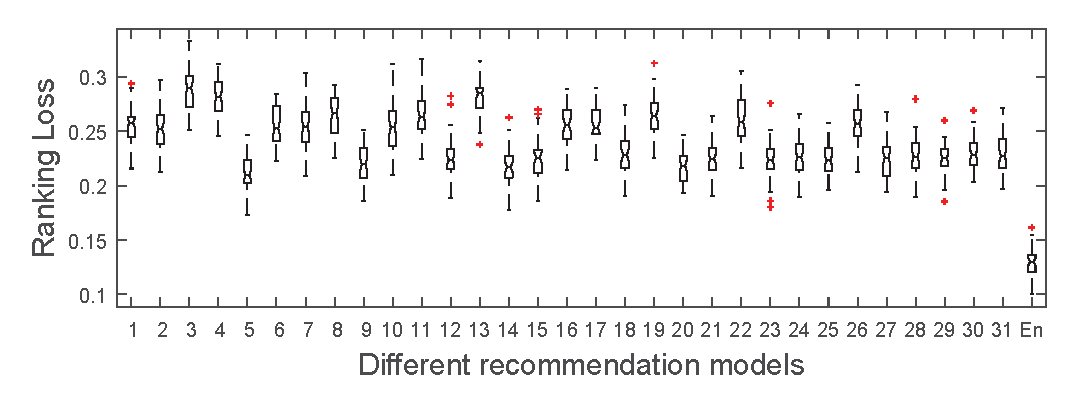
\includegraphics[width=0.95\textwidth]{Figures/RankLossComparison}
	\caption{Comparison betwwen Proposed Ensembel Recommendation Model and 31 Base Recommendation Models in Terms of Ranking Loss}\label{Fig:CompOnHammLoss}
\end{figure}
%==================================================================

\begin{enumerate}
    \item The Ranking Losses of different recommendation models are
    different. And the differences among some models are
    significant. This means that the recommended rankings of candidate algorithms
    vary with different recommendation models. Meanwhile, no matter
    under which kind of combinations of meta-features in Table
    \ref{table:metaFeatureNO}, the recommendation model constructed on the combined meta-features
    performs equally or better than the single kind of
    meta-features. The reason is that different kinds of
    meta-features characterize the classification problems in different
    viewpoints and will be relatively complemented, so the combinations can give us more
    comprehensive understanding of the problem. Furthermore, it is
    possible to construct more precise decision tree model to
    distinguish the appropriate and inappropriate candidate algorithms.

    \item The Ranking Loss of ensemble learning based model (i.e., the last box) is the
    lowest. And it is significantly smaller than that of any other
    recommendation model (i.e., any box numbered by
    $1,2,\cdots,31$). For the other 31 recommendation models, the
    smallest/greatest median value of Ranking Loss is 0.2096/0.2898.
    However, by combining these 31 recommendation models together
    to form the ensemble recommendation model, the median value of
    Ranking Loss is only 0.1301, and outperforms the best base
    recommendation model by 37.93\%. This means that the proposed ensemble learning
    method is more effective to estimate the ranking of the
    candidate algorithms.
\end{enumerate}


\subsubsection{Comparison on Precision}

Fig. \ref{Fig:CompOnMeanPrecision} shows the comparison results of
different recommendations in terms of average precision. From this
figure, we can get that:

%================================================================
\begin{figure}[!h]
	\centering
	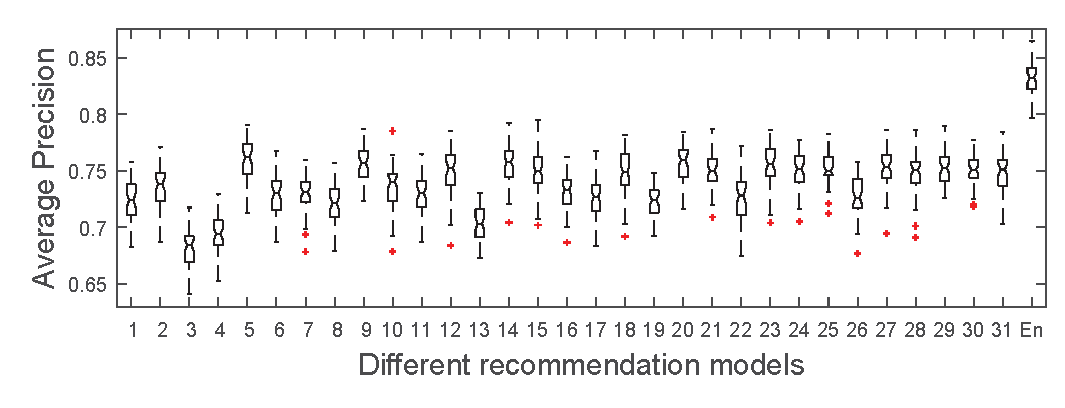
\includegraphics[width=0.95\textwidth]{Figures/MeanPrecisionComparison}
	\caption{Comparison betwwen Proposed Ensembel Recommendation Model and 31 Base Recommendation Models in terms of Average Precision}\label{Fig:CompOnMeanPrecision}
\end{figure}
%==================================================================
\begin{enumerate}
    \item The Average Precision varies with different recommendation
    models. For single kind of meta-features corresponding to the
    first five recommendation models, there exists distinctly
    significant difference among the Average Precision, such as the
    Average Precision of the models constructed on the statistic and
    information theory and structural information based
    meta-features is significantly greater than that of the models
    constructed on other three kinds of meta-features.

    \quad For the models constructed on the different combinations
    of the five kinds of meta-features, their Average Precisions are
    either statistically equal to or greater than that of model
    constructed on the corresponding single kind of meta-features.
    For example, the 13th box corresponds to the Average Precision
    of the model constructed on the combinations of  3rd and 4th
    meta-features. And its median is statistically greater than that of the 3rd box and equal to that of the 4th box.

    \item The Average Precision of ensemble learning based model, which is
    achieved by integrating the 31 recommendation models together, is the
    highest and statistically better than that of any of the other 31
    recommendation models. For the 31 base recommendation models, the
    greatest/smallest median value of Average Precision is 0.7618/0.6839.
    However, by combining these 31 base recommendation models together
    to form the ensemble recommendation model, the median value of
    Average Precision can be up to 0.8324, and outperforms the best base
    recommendation model by 9.27\%. This indicates that combining the
    recommendation models constructed on different sets of
    meta-features together is an effective way to construct the more accurate
    recommendation model.
\end{enumerate}
%==================================================================

%==================================================================
\begin{figure}[!h]
    \centering
    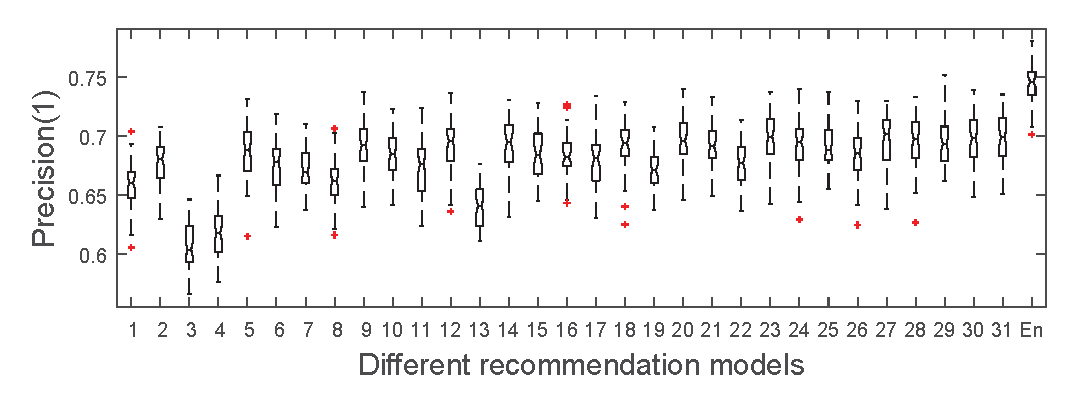
\includegraphics[width=0.95\textwidth]{Figures/FirstPrecisionComparison}
    \caption{Comparison betwwen Proposed Ensembel Recommendation Model and 31 Base Recommendation Models in Terms of Precision(1)}\label{Fig:CompOnPrecision1}
\end{figure}
%==================================================================

Besides the average precision, the user might be interested on the
precision of the top ranked algorithm. That is, whether the first
recommended algorithm is one of the real appropriate algorithms.
This can be measured by the metric \emph{Precision(1)} of the
recommendation model. Fig. \ref{Fig:CompOnPrecision1} shows the
\emph{Precision(1)} of different recommendation models. From Fig.
\ref{Fig:CompOnPrecision1}, we can observe that, the Precision of
the top ranked algorithm recommended by different recommendation
models is different. For the 31 base recommendation models, the
greatest/smallest median value of \emph{Precision(1)} is
0.7016/0.6037. However, by combining these 31 base recommendation
models together to form the ensemble recommendation model, the
median value of \emph{Precision(1)} can be up to 0.7464, and
outperforms the best base recommendation model by 6.39\%.

In summary, no matter in terms of either Average Precision or
\emph{Precision(1)}, the proposed ensemble learning based algorithm
recommendation method is significantly than the existing
recommendation models.

\subsubsection{Comparison with ML-$k$NN Based Recommendation Method}

In this section, we experimentally compare the proposed ensemble
learning based recommendation method with the existing non-ensemble
ML-$k$NN based recommendation
method. Except for constructing recommendation models over the single kind of meta-features as in  in \cite{wang2014generic}, to make a comprehensive
comparison, we also apply the ML-$k$NN based recommendation method
on all the other combinations of the five different kinds of meta-features, where the parameter $k$ is set to be 5 suggested
in \cite{wang2014generic}.

\begin{figure}
    \centering{
    \begin{minipage}{0.95\textwidth}
    {\subfigure[Rank
    Loss]{\label{subfig:rankLoss}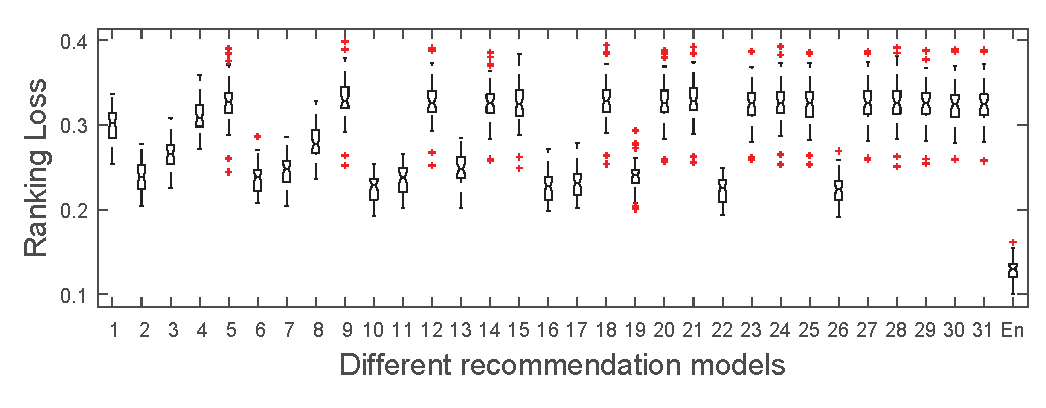
\includegraphics[width=0.95\textwidth]{Figures/KNNRankLoss}}
    \subfigure[Average
    Precision]{\label{subfig:meanPrecision}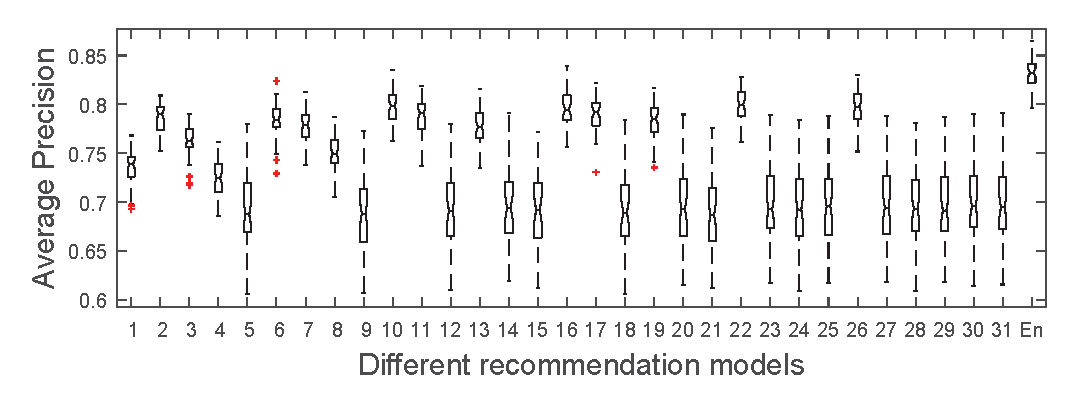
\includegraphics[width=0.95\textwidth]{Figures/KNNAvPrecision}}

    \subfigure[Precision(1)]{\label{subfig:firstPrecision}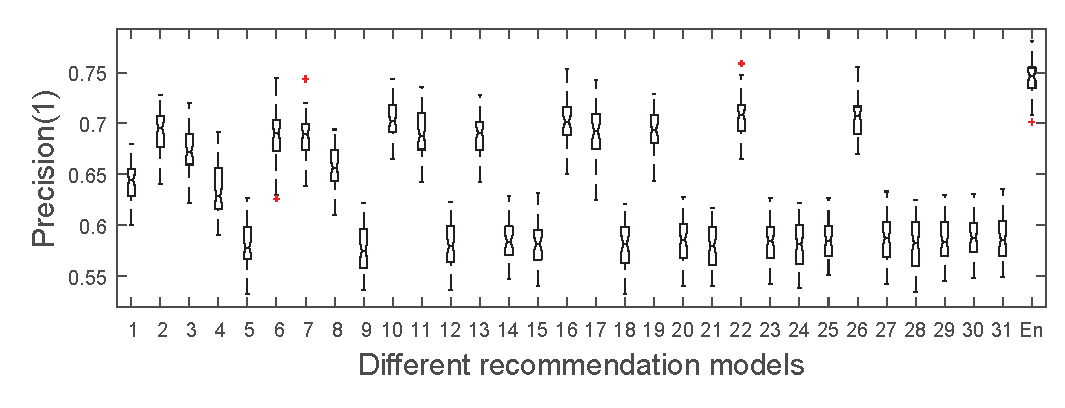
\includegraphics[width=0.95\textwidth]{Figures/KNNFirstPrecision}}}
    \caption{Comparison betwwen Proposed Ensembel Recommendation Model and 31 ML-$k$NN based Recommendation Models}\label{fig:compareToKNN}
    \end{minipage}}
\end{figure}

Fig \ref{fig:compareToKNN} shows the comparison results between the
proposed ensemble method and ML-$k$NN based recommendation method in
terms of \emph{Ranking Loss}, \emph{Average Precision} and
\emph{Precision (1)}, respectively. From this figure, we can observe
that i) the best performance of the recommendation models
constructed by ML-$k$NN is achieved with respect to the combination
of different meta-features rather than a single kind of
meta-features in \cite{wang2014generic}. ii) The ensemble learning
based recommendation model outperforms the existing ML-$k$NN based
one in terms of the median value all these three metrics. The median
value with respect to the ensemble recommendation method outperforms
that the best recommendation model constructed with ML-$k$NN by
41.87\% for \emph{Rank Loss}, 4.10\% for \emph{Average Precision}
and 5.30\% for \emph{Precision(1)}. iii) Comparing Fig.
\ref{subfig:meanPrecision} to Fig. \ref{Fig:CompOnMeanPrecision} in
terms of Average Precision, the most of the ML-$k$NN based
recommendation models in Fig. \ref{subfig:meanPrecision} are
better than the base recommendation models in Fig.
\ref{Fig:CompOnMeanPrecision} with respect to different kinds of
meta-features or combinations. However, by integrating the base
recommendation models in in Fig.
\ref{Fig:CompOnMeanPrecision} together, the ensemble recommendation model
achieves the better performance. This phenomenon can be also
discovered by comparing Fig. \ref{subfig:firstPrecision} to Fig.
\ref{Fig:CompOnPrecision1} in terms of \emph{Precision(1)}. This
indicates that the ensemble learning method proposed in this paper
is quite effective to improve the performance of classification
algorithm recommendation.


\subsubsection{Sensitivity Analysis of Ensemble Recommendation Model}

The necessary and sufficient condition to construct an accurate
ensemble recommendation model is that the base models must be
accurate and diverse. This paper gives the methods to identify the
accurate and diverse learning models. In this section, we give the
sensitivity analysis of how the accurate and diverse models act on
constructing accurate ensemble recommendation model. Fig.
\ref{Fig:sensitiveAnalysis} shows the sensitivity analysis of these
two aspects on the recommendation models in terms of \emph{Ranking
Loss}, \emph{Average Precision}, \emph{Precision(1)} and \emph{the
number of the base models using for ensemble learning},
respectively. In this figure, i) ``all'' represents that all the 31
base recommendation models are used for ensemble model construction;
ii) ``accurate'' denotes the 31 base models are only filtered by the
Definition \ref{def:accurateModel} of accurate learning model; iii)
``diverse'' denotes the 31 base models are only filtered by the
Definition \ref{def:diverseModel} of diverse learning model and iv)
``accurate \& diverse'' means that the 31 base models are filtered
by both Definitions \ref{def:accurateModel} and
\ref{def:diverseModel}.

%==================================================================
\begin{figure}[!h]
	\centering
	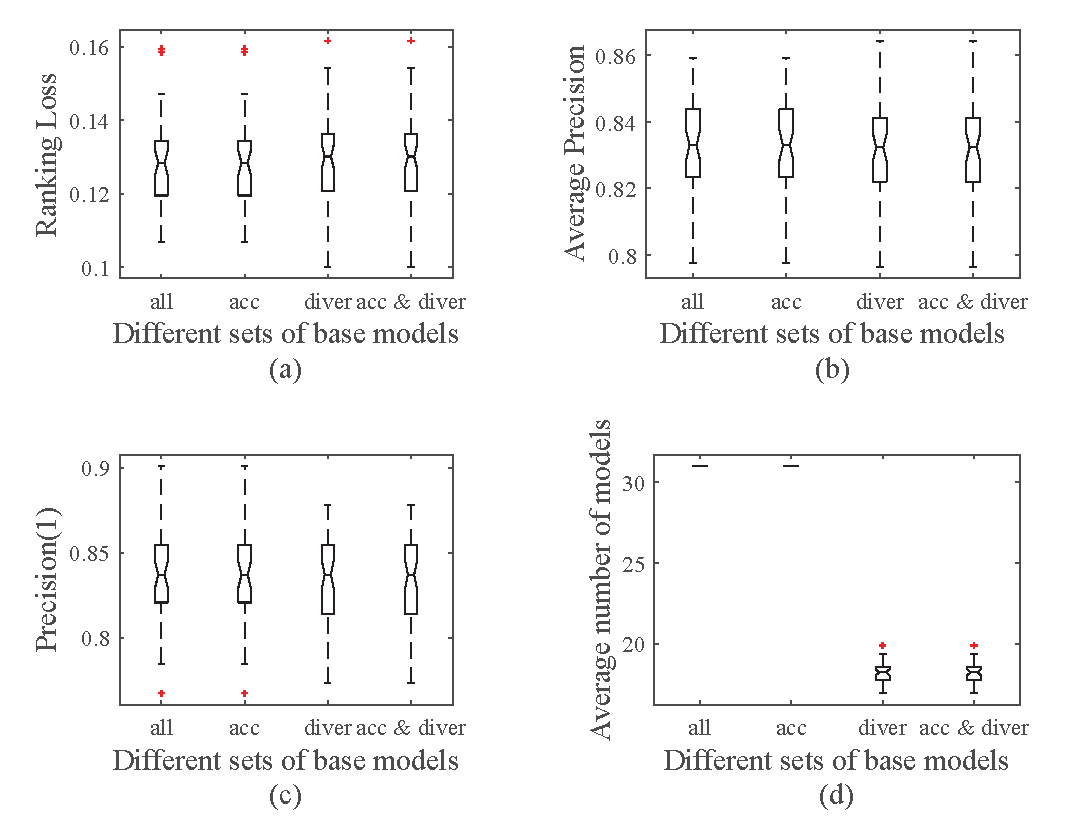
\includegraphics[width=0.85\textwidth]{Figures/SensitiveAnalysis1}
	\caption{Sensitivity Analysis of Accurate and Diverse Models on the Porposed Ensemble Recommendation Model in terms of Ranking Loss, Average Precision, Precision(1) and Number of Base Models}\label{Fig:sensitiveAnalysis}
\end{figure}
%==================================================================

From Fig. \ref{Fig:sensitiveAnalysis}, we can get that:
\begin{enumerate}
    \item For each sub-figure, the four kinds of recommendation models can be grouped into
    two categories according to the box plots of their
    performance metrics. The models marked as ``all'' and ``accurate''
    have statistically equal performance, and the other two models perform
    statistically equally as well.

    \quad This is because that during the base recommendation model
    construction, for all of the single-label learning problems
    transformed from the multi-labeled meta-data by BR
    transformation method, the classification accuracy of decision tree on them is greater
    than 0.5. Therefore, the classification accuracy based filter
    cannot filter out any decision tree. That mean, for
    recommendation models marked as ``all'' and
    ``accurate'', the decision trees used for model construction are
    quite in common. This leads to that the performance of recommendation
    models marked as ``all'' and ``accurate'' are equal.
    Similarly, since the difference among the construction of models
    marked as ``diverse'' and ``accurate \& diverse'' derives from the
    classification accuracy based filter, their performance is
    equal as well. This can be also confirmed by the Fig.
    \ref{Fig:sensitiveAnalysis} (d) showing the average number of
    trees used for ensemble learning based algorithm recommendation.
    The recommendation models marked as ``all'' and ``accurate'' are
    constructed based on the same number of decision trees.
    So the same as the recommendation models marked as ``diverse'' and ``accurate \&
    diverse''.

    \item Since that the most decision trees used for algorithm
    recommendation model constructed are accurate according to
    Definition \ref{def:accurateModel} of accurate learning model,
    the proposed ensemble learning based algorithm recommendation
    method focuses on finding out the diverse base learning
    models. According to Fig. \ref{Fig:sensitiveAnalysis}, after
    filtering out the decision trees by Definition
    \ref{def:diverseModel} of diverse base model, we get better
    ensemble learning based recommendation models with less
    number of decision trees. Such as, the model marked as ``diverse''
    with diversity based filter outperforms the model marked as
    ``all'' in terms of all the performance metrics Ranking Loss,
    Average Precision and Precision(1); and the model marked as
    ``accurate \& diverse'' is better than the model marked as
    ``accurate''. This indicates that $\kappa$ in Eq. \ref{eq:kappa} is a good choice to
    evaluate the diversity between different base models and can
    be used to detect diverse base models for ensemble learning
    based algorithm recommendation.
\end{enumerate}

In summary, by the sensitivity analysis of two important aspects
(including accurate and diverse base learning models) in ensemble
learning model construction, we can conclude that, for
classification algorithm recommendation, the proposed definitions of
accurate and diverse learning models are effective to find out a
good set of base recommendation models to construct better ensemble
recommendation model.


\section{Conclusion}\label{sec:conclusion}

In this paper, we have proposed a novel multi-label ensemble
learning based recommendation method with the aim to support the
automatic recommendation of appropriate classification algorithms
for a new classification problem from a number of candidates.

The proposed method first viewed the algorithm recommendation as a
multi-label learning problem due to the fact that there would be
multiple algorithms being appropriate for a classification problem.
Then, different from the existing recommendation methods which
usually construct the recommendation model on only one kind of
meta-features by a single learner, we constructed the recommendation
model with an ensemble learner which combines a set of base
recommendation models constructed on the combinations of different
kinds of meta-features by tree-based multi-label learners.

Finally, we have thoroughly tested the recommendation method 1723
benchmark classification problems, 17 different classification
algorithms and five different kinds of meta-features. The
experimental results show that the proposed ensemble learning based
recommendation model is more effective.

For future work, as different meta-features play different roles in recommendation model constrution, an intrinuing direction is to concentrate on the feature engineering and inform which meta-features are salient and useful for model construction, and further solve the algorithm recommendation problem in a more efficiently and effectively way.


\appendixhead{Wang}

% Appendix
\appendix\section*{APPENDIX}\setcounter{section}{0}

%\section{Notation of Symbols in the Paper}\label{appendix:symbols}

%========================================================================
\begin{table}[!h]
\centering
    \begin{minipage}{0.85\textwidth}
    \small
    \centering
    \renewcommand{\arraystretch}{0.9}
    \caption{Statistical and Information-Theory Based Measures}\label{tab:statMetrics}
    \resizebox{0.9\textwidth}{!}{
        \begin{tabular}{l|l}
        \hline
        Measures & Definitions\\
        \hline
        Ins.Num & Number of instances\\
        Attr.Num & Number of Attributes\\
        Target.Num & Number of target concept values\\
        Target.Min & Proportion of minority target\\
        Target.Max & Proportion of majority target\\
        Pro.Bin & Proportion of binary attributes\\
        Pro.Nom & Proportion of nominal attributes\\
        Pro.Num & Proportion of numeric attributes\\
        Pro.MissIns & Proportion of instances with missing values\\
        Pro.MissValues & Proportion of missing values\\
        \hline
        Mean.Geo & Geometric mean\\
        Mean.Harm & Harmonic mean\\
        Mean.Trim & Trim mean excluding the highest and lowest 5\%\\
        Mad & Mean absolute deviation\\
        Var & Variance\\
        Std & Standard deviation\\
        Prcitile & Percentile 75\%\\
        Int.Range & Interquartile range\\
        Prop.AttrWithOutlier & Proportion of numerical attributes with outliers over all numerical attributes\\
        Skewness & Skewness of data based on numerical attributes\\
        Kurtosis & Kurtosis of data based on numerical attributes \\
        Max.eig & Maximum eigenvalue\\
        Min.eig & Minimum eigenvalue\\
        Can.corr & Canonical correlation\\
        Grav.cent & Center of gravity\\
        MeanAbsCoef & Mean absolute coefficient of attribute pairs \\
        \hline
        \emph{$H(C)$} & Entropy of classes \\
        \emph{$\bar{H}(X)$} & Mean entropy of nominal attributes \\
        \emph{$\bar{M}(C,X)$} & Mean mutual information of classes and attributes based on nominal attributes\\
        En.attr &  Equivalent number of attributes \emph{$H(C)/\bar{M}(C,X)$}\\
        Ns.ratio & Noise-signal ratio \emph{$\bar{H}(X)/\bar{M}(C,X)-1$} \\
        \hline
        \end{tabular}
    }
    \end{minipage}
    \begin{minipage}{0.85\textwidth}
    \footnotesize
    \centering
    \renewcommand{\arraystretch}{0.9}
    \caption{Model Structure Based Measures}\label{tab:modelMetrics}
    \resizebox{0.9\textwidth}{!}{
        \begin{tabular}{l|l}
        \hline
        Measures & Definitions\\
        \hline
        Tree.Height & Height of tree (also referred as to number of levels in tree)\\
        Tree.Wdith & Width of tree\\
        Node.Num & Number of nodes in tree\\
        Leaf.Num & Number of leaves in tree\\
        \hline
        Level.Max & Maximum number of nodes at one level\\
        Level.Mean & Mean of the number of nodes on levels\\
        Level.Dev & Standard deviation of the number of nodes on levels\\
        \hline
        Branch.Long & Length of the longest branch\\
        Branch.Short & Length of the shortest branch\\
        Branch.Mean & Mean of the branch lengths\\
        Branch.Dev & Standard deviation of the branch lengths\\
        \hline
        Attr.Min & Minimum occurrence of attributes\\
        Attr.Max & Maximum occurrence of attributes\\
        Attr.Mean & Mean of the number of occurrences of attributes\\
        Attr.Dev & Standard deviation of the number of occurrences of attributes\\
        \hline
        \end{tabular}
    }
    \end{minipage}
    \begin{minipage}{0.85\textwidth}
    \footnotesize
    \centering
    \renewcommand{\arraystretch}{0.9}
    \caption{Problem Complexity Based Measures}\label{tab:complexityMetrics}
    \resizebox{0.9\textwidth}{!}{
        \begin{tabular}{l|l}
        \hline
        Measures & Definitions\\
        \hline
        Bound.Len & Length of class boundary \\
        Adherence.Prop &  Proportion of retained adherence subsets\\
        Intra/Inter.Ratio &  Ratio of average intra/interclass nearest neighbors \\
        NN.Nonlinerity &  Nonlinearity of Nearest Neighbors classifier \\
        Linear.Nonlinerity & Nonlinearity of linear classifier \\
        Fisher.Ratio & Maximum Fisher's discriminant ratio \\
        Ins/Attr & Training set size relative to feature space dimensionality \\
        \hline
        \end{tabular}
    }
    \end{minipage}
\end{table}
%========================================================================

\section{Five Different Kinds of Meta-features for Algorithm Recommendation}\label{appendix:metaFeature}

\begin{enumerate}
    \item {Statistical and Information-Theory Based Measures} (See Table \ref{tab:statMetrics})

    The statistical and information-theory based measures are the most
    widely-used in the filed of algorithm recommendation
    \cite{brazdil2003ranking,king1995statlog,sohn1999meta,Henery1995methods,aha1992generalizing}.
    The prominent examples based on these measures are the projects
    ESPRIT Statlog (1991-1994) and METAL (1998-2001). These measures
    generally include the data set characteristics such as, number of
    features, number of instances, number of target concepts, ratio of
    instances to features, ratio of missing values, ratio of binary
    features, entropy of the target concept, information gain between
    the feature and the target concept, and correlation coefficient
    between features, etc.

    \item {Model Structure Based Measures} (See Table \ref{tab:modelMetrics})

    For this kind of measures, a learning problem is represented in a
    special data structure which can embed the complexity of a problem.
    Then, the characteristics of the structure are exploited to describe
    the learning problem.

    \quad In the field of algorithm recommendation, the induced decision
    tree is a well-known and commonly-used structure to model a learning
    problem. Bensusan \citeyear{Bensusan1998god} proposed to capture the
    information from the induced decision tree for describing the
    learning complexity. He extracted ten measures from the decision
    tree, such as the ratio of the number of nodes to the number of
    features, the ratio of the number of nodes to the number of
    instances, etc. Afterwards, Peng et al. \citeyear{peng2002improved}
    re-analyzed the characterization of decision trees, and proposed
    some new measures to characterize the structural properties of
    decision trees.

    \item {Landmarking Based Measures}

    This kind of measures falls within the concept of landmarking
    \cite{Pfahringer00meta,Bensusan2000casa,jain2000statistical,duin2004characterization}.
    This idea was proposed based on the assumption that the performance
    of the candidate algorithms could be predicted by the performance of
    a set of simple learners (also called landmarkers). The performance
    (e.g., accuracy) of these landmarkers is used to describe a learning
    problem. Evidently, this kind of measures depends on the choice of
    landmarkers. In practice, it should be ensured that the chosen
    landmarkers have significant differences in terms of learning
    mechanism.

    \quad Following the suggestions in
    \cite{Pfahringer00meta,Bensusan2000casa}, the following six classifiers are
    selected as the landmark learners: i) Naive Bayes, ii) 1-NN (Nearest Neighbor),
    iii) Elite 1-NN, iv) a decision node learner, v)
    a random chosen node learner and  vi) the worst node learner.
    Where the last three learners can be achieved based on the
    well-known learning algorithm C4.5.

    \item {Problem Complexity Based Measures} (See Table
    \ref{tab:complexityMetrics})

    In addition to the above problem characterization methods, the
    problem complexity based measures also were exploited to describe
    the learning problems in
    \cite{bernado2005domain,ho2002complexity,elizondo2009estimation,ho2000complexity}.
    By analyzing the source of difficulty in solving a learning problem,
    they focus on the description of the geometrical complexity of the
    problem and emphasize the geometrical characteristics of the
    distributions of the classes. The features reflecting the way in
    which different classes are separated or interleaved (and being
    relevant to learning performance) are identified as the measurement
    of the problem's complexity.

    \item {Structural Information Based Measures}

    Recently, Song et al. proposed a novel problem characterization
    method to facilitate the algorithm recommendation
    \cite{song2012automatic}. The method uses structural information
    based feature vectors to characterize the learning problems, which
    is quite different from the existing ones. Specially, the two
    feature vectors, one-item feature vector and two-item feature
    vector, are extracted from the given problem at first. These two vectors
    consists the frequencies of one-item sets and two-item sets,
    respectively. Afterward, the \emph{minimum}, \emph{1/8
    quantile}, \emph{2/8 quantile}, \emph{3/8 quantile}, \emph{4/8
    quantile}, \emph{5/8 quantile}, \emph{6/8 quantile}, \emph{7/8
    quantile} and \emph{maximum} are computed for these two vectors
    and form the final set of data set characteristics.
\end{enumerate}

% Acknowledgments
\begin{acks}
The authors would like to the editors and the anonymous reviewers for their insightful and helpful comments and suggestions, which resulted in substantial improvements to this work. This work is supported by the National Natural Science Foundation of China (Grant No. 61502378, 61402355), the Postdoctoral Science Foundation of China (Grant No. 2014M562417), the Program of State Key Software Engineering Laboratory, Wuhan University, China (Grant No. 2015Program17) and the Shaanxi Province Postdoctoral Sustentation Fund, China.
\end{acks}

% Bibliography
\bibliographystyle{acmsmall}
\bibliography{AlgRecOnEnsemble}

% %History dates
%\received{February 2007}{March 2009}{June 2009}
%
%% Electronic Appendix
%\elecappendix

%\medskip
%
%\section{This is an example of Appendix section head}
%
%Channel-switching time is measured as the time length it takes for
%motes to successfully switch from one channel to another. This
%parameter impacts the maximum network throughput, because motes
%cannot receive or send any packet during this period of time, and it
%also affects the efficiency of toggle snooping in MMSN, where motes
%need to sense through channels rapidly.
%
%By repeating experiments 100 times, we get the average
%channel-switching time of Micaz motes: 24.3 $\mu$s. We then conduct
%the same experiments with different Micaz motes, as well as
%experiments with the transmitter switching from Channel 11 to other
%channels. In both scenarios, the channel-switching time does not have
%obvious changes. (In our experiments, all values are in the range of
%23.6 $\mu$s to 24.9 $\mu$s.)
%
%\section{Appendix section head}
%
%The primary consumer of energy in WSNs is idle listening. The key to
%reduce idle listening is executing low duty-cycle on nodes. Two
%primary approaches are considered in controlling duty-cycles in the
%MAC layer.

\end{document}
